\documentclass[output=paper,hidelinks]{langscibook}
\ChapterDOI{10.5281/zenodo.10185989}
\title{Treebank-driven parsing, translation and grammar induction using LFG}
\author{Aoife Cahill\affiliation{Educational Testing Service} and Andy Way\affiliation{ADAPT Centre, School of Computing, Dublin City University}}
\abstract{This chapter provides a summary of a range of work on probabilistic models of Lexical Functional Grammar (LFG).  LFG grammars as originally conceived in  \citet{kaplanbresnan82} were defined by grammatical rules and constraints, so could not describe ill-formed strings, and they failed if confronted with well-formed strings outside their coverage. In contrast, the hybrid LFG-DOP model of \cite{bod-kaplan-1998-probabilistic-corpus} and \cite{BK2003} could   generalize well-formed analyses via the  {\em Discard} operation   to allow ill-formed and previously uncovered well-formed strings to be handled.      \citet{Way99} and \citet{Way01} extended LFG-DOP to handle translation, and demonstrated two advantages of his LFG-DOT models: (i) being probabilistic, LFG-DOT was able to handle a range of translation phenomena that were problematic for the description of LFG-MT \citep{kaplanetal1989}; and (ii) having f-structure constraints enabled LFG-DOT to overcome problems for DOT \citep{DOT}, a model of translation based on DOP \citep{Bod92,Simaan95,Bod98}.    Like most probabilistic models, LFG-DOP (and LFG-DOT) require large  amounts of annotated data. In a range of seminal work on grammar  induction -- now a research field in its own right, but at the time quite a novelty -- it was demonstrated how strings could be  automatically annotated with both LFG c- and f-structure  information \citep{S-vG-W-00,Cahill02automatic}. These were then used for multilingual probabilistic   parsing \citep{cahill2005multilingual,cahill-etal-2008-wide} and lexicon induction experiments \citep{odonovan:2006}, which we describe here.}

\IfFileExists{../localcommands.tex}{
   \addbibresource{../localbibliography.bib}
   \addbibresource{thisvolume.bib}
   % add all extra packages you need to load to this file

\usepackage{tabularx}
\usepackage{multicol}
\usepackage{url}
\urlstyle{same}
%\usepackage{amsmath,amssymb}

% Tight underlining according to https://alexwlchan.net/2017/10/latex-underlines/
\usepackage{contour}
\usepackage[normalem]{ulem}
\renewcommand{\ULdepth}{1.8pt}
\contourlength{0.8pt}
\newcommand{\tightuline}[1]{%
  \uline{\phantom{#1}}%
  \llap{\contour{white}{#1}}}
  
\usepackage{listings}
\lstset{basicstyle=\ttfamily,tabsize=2,breaklines=true}

% \usepackage{langsci-basic}
\usepackage{langsci-optional}
\usepackage[danger]{langsci-lgr}
\usepackage{langsci-gb4e}
%\usepackage{langsci-linguex}
%\usepackage{langsci-forest-setup}
\usepackage[tikz]{langsci-avm} % added tikz flag, 29 July 21
% \usepackage{langsci-textipa}

\usepackage[linguistics,edges]{forest}
\usepackage{tikz-qtree}
\usetikzlibrary{positioning, tikzmark, arrows.meta, calc, matrix, shapes.symbols}
\usetikzlibrary{arrows, arrows.meta, shapes, chains, decorations.text}

%%%%%%%%%%%%%%%%%%%%% Packages for all chapters

% arrows and lines between structures
\usepackage{pst-node}

% lfg attributes and values, lines (relies on pst-node), lexical entries, phrase structure rules
\usepackage{packages/lfg-abbrevs}

% subfigures
\usepackage{subcaption}

% macros for small illustrations in the glossary
\usepackage{./packages/picins}

%%%%%%%%%%%%%%%%%%%%% Packages from contributors

% % Simpler Syntax packages
\usepackage{bm}
\tikzstyle{block} = [rectangle, draw, text width=5em, text centered, minimum height=3em]
\tikzstyle{line} = [draw, thick, -latex']

% Dependency packages
\usepackage{tikz-dependency}
%\usepackage{sdrt}

\usepackage{soul}

\usepackage[notipa]{ot-tableau}

% Historical
\usepackage{stackengine}
\usepackage{bigdelim}

% Morphology
\usepackage{./packages/prooftree}
\usepackage{arydshln}
\usepackage{stmaryrd}

% TAG
\usepackage{pbox}

\usepackage{langsci-branding}

   % %%%%%%%%% lang sci press commands

\newcommand*{\orcid}{}

\makeatletter
\let\thetitle\@title
\let\theauthor\@author
\makeatother

\newcommand{\togglepaper}[1][0]{
   \bibliography{../localbibliography}
   \papernote{\scriptsize\normalfont
     \theauthor.
     \titleTemp.
     To appear in:
     Dalrymple, Mary (ed.).
     Handbook of Lexical Functional Grammar.
     Berlin: Language Science Press. [preliminary page numbering]
   }
   \pagenumbering{roman}
   \setcounter{chapter}{#1}
   \addtocounter{chapter}{-1}
}

\DeclareOldFontCommand{\rm}{\normalfont\rmfamily}{\mathrm}
\DeclareOldFontCommand{\sf}{\normalfont\sffamily}{\mathsf}
\DeclareOldFontCommand{\tt}{\normalfont\ttfamily}{\mathtt}
\DeclareOldFontCommand{\bf}{\normalfont\bfseries}{\mathbf}
\DeclareOldFontCommand{\it}{\normalfont\itshape}{\mathit}
\makeatletter
\DeclareOldFontCommand{\sc}{\normalfont\scshape}{\@nomath\sc}
\makeatother

% Bug fix, 3 April 2021
\SetupAffiliations{output in groups = false,
                   separator between two = {\bigskip\\},
                   separator between multiple = {\bigskip\\},
                   separator between final two = {\bigskip\\}
                   }

% commands for all chapters
\setmathfont{LibertinusMath-Additions.otf}[range="22B8]

% punctuation between a sequence of years in a citation
% OLD: \renewcommand{\compcitedelim}{\multicitedelim}
\renewcommand{\compcitedelim}{\addcomma\space}

% \citegen with no parentheses around year
\providecommand{\citegenalt}[2][]{\citeauthor{#2}'s \citeyear*[#1]{#2}}

% avms with plain font, using langsci-avm package
\avmdefinestyle{plain}{attributes=\normalfont,values=\normalfont,types=\normalfont,extraskip=0.2em}
% avms with attributes and values in small caps, using langsci-avm package
\avmdefinestyle{fstr}{attributes=\scshape,values=\scshape,extraskip=0.2em}
% avms with attributes in small caps, values in plain font (from peter sells)
\avmdefinestyle{fstr-ps}{attributes=\scshape,values=\normalfont,extraskip=0.2em}

% reference to previous or following examples, from Stefan
%(\mex{1}) is like \next, referring to the next example
%(\mex{0}) is like \last, referring to the previous example, etc
\makeatletter
\newcommand{\mex}[1]{\the\numexpr\c@equation+#1\relax}
\makeatother

% do not add xspace before these
\xspaceaddexceptions{1234=|*\}\restrict\,}

% Several chapters use evnup -- this is verbatim from lingmacros.sty
\makeatletter
\def\evnup{\@ifnextchar[{\@evnup}{\@evnup[0pt]}}
\def\@evnup[#1]#2{\setbox1=\hbox{#2}%
\dimen1=\ht1 \advance\dimen1 by -.5\baselineskip%
\advance\dimen1 by -#1%
\leavevmode\lower\dimen1\box1}
\makeatother

% Centered entries in tables.  Requires array package.
\newcolumntype{P}[1]{>{\centering\arraybackslash}p{#1}}

% Reference to multiple figures, requested by Victoria Rosen
\newcommand{\figsref}[2]{Figures~\ref{#1}~and~\ref{#2}}
\newcommand{\figsrefthree}[3]{Figures~\ref{#1},~\ref{#2}~and~\ref{#3}}
\newcommand{\figsreffour}[4]{Figures~\ref{#1},~\ref{#2},~\ref{#3}~and~\ref{#4}}
\newcommand{\figsreffive}[5]{Figures~\ref{#1},~\ref{#2},~\ref{#3},~\ref{#4}~and~\ref{#5}}

% Semitic chapter:
\providecommand{\textchi}{χ}

% Prosody chapter
\makeatletter
\providecommand{\leftleadsto}{%
  \mathrel{\mathpalette\reflect@squig\relax}%
}
\newcommand{\reflect@squig}[2]{%
  \reflectbox{$\m@th#1$$\leadsto$}%
}
\makeatother
\newcommand\myrotaL[1]{\mathrel{\rotatebox[origin=c]{#1}{$\leadsto$}}}
\newcommand\Prosleftarrow{\myrotaL{-135}}
\newcommand\myrotaR[1]{\mathrel{\rotatebox[origin=c]{#1}{$\leftleadsto$}}}
\newcommand\Prosrightarrow{\myrotaR{135}}

% Core Concepts chapter
\newcommand{\anterm}[2]{#1\\#2}
\newcommand{\annode}[2]{#1\\#2}

% HPSG chapter
\newcommand{\HPSGphon}[1]{〈#1〉}
% for defining RSRL relations:
\newcommand{\HPSGsfl}{\enskip\ensuremath{\stackrel{\forall{}}{\Longleftarrow{}}}\enskip}
% AVM commands, valid only inside \avm{}
\avmdefinecommand {phon}[phon] { attributes=\itshape } % define a new \phon command
% Forest Set-up
\forestset
  {notin label above/.style={edge label={node[midway,sloped,above,inner sep=0pt]{\strut$\ni$}}},
    notin label below/.style={edge label={node[midway,sloped,below,inner sep=0pt]{\strut$\ni$}}},
  }

% Dependency chapter
\newcommand{\ua}{\ensuremath{\uparrow}}
\newcommand{\da}{\ensuremath{\downarrow}}
\forestset{
  dg edges/.style={for tree={parent anchor=south, child anchor=north,align=center,base=bottom},
                 where n children=0{tier=word,edge=dotted,calign with current edge}{}
                },
dg transfer/.style={edge path={\noexpand\path[\forestoption{edge}, rounded corners=3pt]
    % the line downwards
    (!u.parent anchor)-- +($(0,-l)-(0,4pt)$)-- +($(12pt,-l)-(0,4pt)$)
    % the horizontal line
    ($(!p.north west)+(0,l)-(0,20pt)$)--($(.north east)+(0,l)-(0,20pt)$)\forestoption{edge label};},!p.edge'={}},
% for Tesniere-style junctions
dg junction/.style={no edge, tikz+={\draw (!p.east)--(!.west) (.east)--(!n.west);}    }
}


% Glossary
\makeatletter % does not work with \newcommand
\def\namedlabel#1#2{\begingroup
   \def\@currentlabel{#2}%
   \phantomsection\label{#1}\endgroup
}
\makeatother


\renewcommand{\textopeno}{ɔ}
\providecommand{\textepsilon}{ɛ}

\renewcommand{\textbari}{ɨ}
\renewcommand{\textbaru}{ʉ}
\newcommand{\acutetextbari}{í̵}
\renewcommand{\textlyoghlig}{ɮ}
\renewcommand{\textdyoghlig}{ʤ}
\renewcommand{\textschwa}{ə}
\renewcommand{\textprimstress}{ˈ}
\newcommand{\texteng}{ŋ}
\renewcommand{\textbeltl}{ɬ}
\newcommand{\textramshorns}{ɤ}

\newbool{bookcompile}
\booltrue{bookcompile}
\newcommand{\bookorchapter}[2]{\ifbool{bookcompile}{#1}{#2}}




\renewcommand{\textsci}{ɪ}
\renewcommand{\textturnscripta}{ɒ}

\renewcommand{\textscripta}{ɑ}
\renewcommand{\textteshlig}{ʧ}
\providecommand{\textupsilon}{υ}
\renewcommand{\textyogh}{ʒ}
\newcommand{\textpolhook}{̨}

\renewcommand{\sectref}[1]{Section~\ref{#1}}

%\KOMAoptions{chapterprefix=true}

\renewcommand{\textturnv}{ʌ}
\renewcommand{\textrevepsilon}{ɜ}
\renewcommand{\textsecstress}{ˌ}
\renewcommand{\textscriptv}{ʋ}
\renewcommand{\textglotstop}{ʔ}
\renewcommand{\textrevglotstop}{ʕ}
%\newcommand{\textcrh}{ħ}
\renewcommand{\textesh}{ʃ}

% label for submitted and published chapters
\newcommand{\submitted}{{\color{red}Final version submitted to Language Science Press.}}
\newcommand{\published}{{\color{red}Final version published by
    Language Science Press, available at \url{https://langsci-press.org/catalog/book/312}.}}

% Treebank definitions
\definecolor{tomato}{rgb}{0.9,0,0}
\definecolor{kelly}{rgb}{0,0.65,0}

% Minimalism chapter
\newcommand\tr[1]{$<$\textcolor{gray}{#1}$>$}
\newcommand\gapline{\lower.1ex\hbox to 1.2em{\bf \ \hrulefill\ }}
\newcommand\cnom{{\llap{[}}Case:Nom{\rlap{]}}}
\newcommand\cacc{{\llap{[}}Case:Acc{\rlap{]}}}
\newcommand\tpres{{\llap{[}}Tns:Pres{\rlap{]}}}
\newcommand\fstackwe{{\llap{[}}Tns:Pres{\rlap{]}}\\{\llap{[}}Pers:1{\rlap{]}}\\{\llap{[}}Num:Pl{\rlap{]}}}
\newcommand\fstackone{{\llap{[}}Tns:Past{\rlap{]}}\\{\llap{[}}Pers:\ {\rlap{]}}\\{\llap{[}}Num:\ {\rlap{]}}}
\newcommand\fstacktwo{{\llap{[}}Pers:3{\rlap{]}}\\{\llap{[}}Num:Pl{\rlap{]}}\\{\llap{[}}Case:\ {\rlap{]}}}
\newcommand\fstackthr{{\llap{[}}Tns:Past{\rlap{]}}\\{\llap{[}}Pers:3{\rlap{]}}\\{\llap{[}}Num:Pl{\rlap{]}}} 
\newcommand\fstackfou{{\llap{[}}Pers:3{\rlap{]}}\\{\llap{[}}Num:Pl{\rlap{]}}\\{\llap{[}}Case:Nom{\rlap{]}}}
\newcommand\fstackonefill{{\llap{[}}Tns:Past{\rlap{]}}\\{\llap{[}}Pers:3{\rlap{]}}\\%
  {\llap{[}}Num:Pl{\rlap{]}}}
\newcommand\fstackoneint%
    {{\llap{[}}{\bf Tns:Past}{\rlap{]}}\\{\llap{[}}Pers:\ {\rlap{]}}\\{\llap{[}}Num:\ {\rlap{]}}}
\newcommand\fstacktwoint%
    {{\llap{[}}{\bf Pers:3}{\rlap{]}}\\{\llap{[}}{\bf Num:Pl}{\rlap{]}}\\{\llap{[}}Case:\ {\rlap{]}}}
\newcommand\fstackthrchk%
    {{\llap{[}}{\bf Tns:Past}{\rlap{]}}\\{\llap{[}}{Pers:3}{\rlap{]}}\\%
      {\llap{[}}Num:Pl{\rlap{]}}} 
\newcommand\fstackfouchk%
    {{\llap{[}}{\bf Pers:3}{\rlap{]}}\\{\llap{[}}{\bf Num:Pl}{\rlap{]}}\\%
      {\llap{[}}Case:Nom{\rlap{]}}}
\newcommand\uinfl{{\llap{[}}Infl:\ \ {\rlap{]}}}
\newcommand\inflpass{{\llap{[}}Infl:Pass{\rlap{]}}}
\newcommand\fepp{{\llap{[}}EPP{\rlap{]}}}
\newcommand\sepp{{\llap{[}}\st{EPP}{\rlap{]}}}
\newcommand\rdash{\rlap{\hbox to 24em{\hfill (dashed lines represent
      information flow)}}}


% Computational chapter
\usepackage{./packages/kaplan}
\renewcommand{\red}{\color{lsLightWine}}

% Sinitic
\newcommand{\FRAME}{\textsc{frame}\xspace}
\newcommand{\arglistit}[1]{{\textlangle}\textit{#1}{\textrangle}}

%WestGermanic
\newcommand{\streep}[1]{\mbox{\rule{1pt}{0pt}\rule[.5ex]{#1}{.5pt}\rule{-1pt}{0pt}\rule{-#1}{0pt}}}

\newcommand{\hspaceThis}[1]{\hphantom{#1}}


\newcommand{\FIG}{\textsc{figure}}
\newcommand{\GR}{\textsc{ground}}

%%%%% Morphology
% Single quote
\newcommand{\asquote}[1]{`{#1}'} % Single quotes
\newcommand{\atrns}[1]{\asquote{#1}} % Translation
\newcommand{\attrns}[1]{(\asquote{#1})} % Translation
\newcommand{\ascare}[1]{\asquote{#1}} % Scare quotes
\newcommand{\aqterm}[1]{\asquote{#1}} % Quoted terms
% Double quote
\newcommand{\adquote}[1]{``{#1}''} % Double quotes
\newcommand{\aquoot}[1]{\adquote{#1}} % Quotes
% Italics
\newcommand{\aword}[1]{\textit{#1}}  % mention of word
\newcommand{\aterm}[1]{\textit{#1}}
% Small caps
\newcommand{\amg}[1]{{\textsc{\MakeLowercase{#1}}}}
\newcommand{\ali}[1]{\MakeLowercase{\textsc{#1}}}
\newcommand{\feat}[1]{{\textsc{#1}}}
\newcommand{\val}[1]{\textsc{#1}}
\newcommand{\pred}[1]{\textsc{#1}}
\newcommand{\predvall}[1]{\textsc{#1}}
% Misc commands
\newcommand{\exrr}[2][]{(\ref{ex:#2}{#1})}
\newcommand{\csn}[3][t]{\begin{tabular}[#1]{@{\strut}c@{\strut}}#2\\#3\end{tabular}}
\newcommand{\sem}[2][]{\ensuremath{\left\llbracket \mbox{#2} \right\rrbracket^{#1}}}
\newcommand{\apf}[2][\ensuremath{\sigma}]{\ensuremath{\langle}#2,#1\ensuremath{\rangle}}
\newcommand{\formula}[2][t]{\ensuremath{\begin{array}[#1]{@{\strut}l@{\strut}}#2%
                                         \end{array}}}
\newcommand{\Down}{$\downarrow$}
\newcommand{\Up}{$\uparrow$}
\newcommand{\updown}{$\uparrow=\downarrow$}
\newcommand{\upsigb}{\mbox{\ensuremath{\uparrow\hspace{-0.35em}_\sigma}}}
\newcommand{\lrfg}{L\textsubscript{R}FG} 
\newcommand{\dmroot}{\ensuremath{\sqrt{\hspace{1em}}}}
\newcommand{\amother}{\mbox{\ensuremath{\hat{\raisebox{-.25ex}{\ensuremath{\ast}}}}}}
\newcommand{\expone}{\ensuremath{\xrightarrow{\nu}}}
\newcommand{\sig}{\mbox{$_\sigma\,$}}
\newcommand{\aset}[1]{\{#1\}}
\newcommand{\linimp}{\mbox{\ensuremath{\,\multimap\,}}}
\newcommand{\fsfunc}{\ensuremath{\Phi}\hspace*{-.15em}}
\newcommand{\cons}[1]{\ensuremath{\mbox{\textbf{\textup{#1}}}}}
\newcommand{\amic}[1][]{\cons{MostInformative$_c$}{#1}}
\newcommand{\amif}[1][]{\cons{MostInformative$_f$}{#1}}
\newcommand{\amis}[1][]{\cons{MostInformative$_s$}{#1}}
\newcommand{\amsp}[1][]{\cons{MostSpecific}{#1}}

%Glue
\newcommand{\glues}{Glue Semantics} % macro for consistency
\newcommand{\glue}{Glue} % macro for consistency
\newcommand{\lfgglue}{LFG$+$Glue} 
\newcommand{\scare}[1]{`{#1}'} % Scare quotes
\newcommand{\word}[1]{\textit{#1}}  % mention of word
\newcommand{\dquote}[1]{``{#1}''} % Double quotes
\newcommand{\high}[1]{\textit{#1}} % highlight (italicize)
\newcommand{\laml}{{L}} 
% Left interpretation double bracket
\newcommand{\Lsem}{\ensuremath{\left\llbracket}} 
% Right interpretation double bracket
\newcommand{\Rsem}{\ensuremath{\right\rrbracket}} 
\newcommand{\nohigh}[1]{{#1}} % nohighlight (regular font)
% Linear implication elimination
\newcommand{\linimpE}{\mbox{\small\ensuremath{\multimap_{\mathcal{E}}}}}
% Linear implication introduction, plain
\newcommand{\linimpI}{\mbox{\small\ensuremath{\multimap_{\mathcal{I}}}}}
% Linear implication introduction, with flag
\newcommand{\linimpIi}[1]{\mbox{\small\ensuremath{\multimap_{{\mathcal{I}},#1}}}}
% Linear universal elimination
\newcommand{\forallE}{\mbox{\small\ensuremath{\forall_{{\mathcal{E}}}}}}
% Tensor elimination
\newcommand{\tensorEij}[2]{\mbox{\small\ensuremath{\otimes_{{\mathcal{E}},#1,#2}}}}
% CG forward slash
\newcommand{\fs}{\ensuremath{/}} 
% s-structure mapping, no space after                                     
\newcommand{\sigb}{\mbox{$_\sigma$}}
% uparrow with s-structure mapping, with small space after  
\newcommand{\upsig}{\mbox{\ensuremath{\uparrow\hspace{-0.35em}_\sigma\,}}}
\newcommand{\fsa}[1]{\textit{#1}}
\newcommand{\sqz}[1]{#1}
% Angled brackets (types, etc.)
\newcommand{\bracket}[1]{\ensuremath{\left\langle\mbox{\textit{#1}}\right\rangle}}
% glue logic string term
\newcommand{\gterm}[1]{\ensuremath{\mbox{\textup{\textit{#1}}}}}
% abstract grammatical formative
\newcommand{\gform}[1]{\ensuremath{\mbox{\textsc{\textup{#1}}}}}
% let
\newcommand{\llet}[3]{\ensuremath{\mbox{\textsf{let}}~{#1}~\mbox{\textsf{be}}~{#2}~\mbox{\textsf{in}}~{#3}}}
% Word-adorned proof steps
\providecommand{\vformula}[2]{%
  \begin{array}[b]{l}
    \mbox{\textbf{\textit{#1}}}\\%[-0.5ex]
    \formula{#2}
  \end{array}
}

%TAG
\newcommand{\fm}[1]{\textsc{#1}}
\newcommand{\struc}[1]{{#1-struc\-ture}}
\newcommand{\func}[1]{\mbox{#1-function}}
\newcommand{\fstruc}{\struc{f}}
\newcommand{\cstruc}{\struc{c}}
\newcommand{\sstruc}{\struc{s}}
\newcommand{\astruc}{\struc{a}}
\newcommand{\nodelabels}[2]{\rlap{\ensuremath{^{#1}_{#2}}}}
\newcommand{\footnode}{\rlap{\ensuremath{^{*}}}}
\newcommand{\nafootnode}{\rlap{\ensuremath{^{*}_{\nalabel}}}}
\newcommand{\nanode}{\rlap{\ensuremath{_{\nalabel}}}}
\newcommand{\AdjConstrText}[1]{\textnormal{\small #1}}
\newcommand{\nalabel}{\AdjConstrText{NA}}

%Case
\newcommand{\MID}{\textsc{mid}{}\xspace}

%font commands added April 2023 for Control and Case chapters
\def\textthorn{þ}
\def\texteth{ð}
\def\textinvscr{ʁ}
\def\textcrh{ħ}
\def\textgamma{ɣ}

% Coordination
\newcommand{\CONJ}{\textsc{conj}{}\xspace}
\newcommand*{\phtm}[1]{\setbox0=\hbox{#1}\hspace{\wd0}}
\newcommand{\ggl}{\hfill(Google)}
\newcommand{\nkjp}{\hfill(NKJP)}

% LDDs
\newcommand{\ubd}{\attr{ubd}\xspace}
% \newcommand{\disattr}[1]{\blue \attr{#1}}  % on topic/focus path
% \newcommand{\proattr}[1]{\green\attr{#1}}  % On Q/Relpro path
\newcommand{\disattr}[1]{\color{lsMidBlue}\attr{#1}}  % on topic/focus path
\newcommand{\proattr}[1]{\color{lsMidGreen}\attr{#1}}  % On Q/Relpro path
\newcommand{\eestring}{\mbox{$e$}\xspace}
\providecommand{\disj}[1]{\{\attr{#1}\}}
\providecommand{\estring}{\mb{\epsilon}}
\providecommand{\termcomp}[1]{\attr{\backslash {#1}}}
\newcommand{\templatecall}[2]{{\small @}(\attr{#1}\ \attr{#2})}
\newcommand{\xlgf}[1]{(\leftarrow\ \attr{#1})} 
\newcommand{\xrgf}[1]{(\rightarrow\ \attr{#1})}
\newcommand{\rval}[2]{\annobox {\xrgf{#1}\teq\attr{#2}}}
\newcommand{\memb}[1]{\annobox {\downarrow\, \in \xugf{#1}}}
\newcommand{\lgf}[1]{\annobox {\xlgf{#1}}}
\newcommand{\rgf}[1]{\annobox {\xrgf{#1}}}
\newcommand{\rvalc}[2]{\annobox {\xrgf{#1}\teqc\attr{#2}}}
\newcommand{\xgfu}[1]{(\attr{#1}\uparrow)}
\newcommand{\gfu}[1]{\annobox {\xgfu{#1}}}
\newcommand{\nmemb}[3]{\annobox {{#1}\, \in \ngf{#2}{#3}}}
\newcommand{\dgf}[1]{\annobox {\xdgf{#1}}}
\newcommand{\predsfraise}[3]{\annobox {\xugf{pred}\teq\semformraise{#1}{#2}{#3}}}
\newcommand{\semformraise}[3]{\annobox {\textrm{`}\hspace{-.05em}\attr{#1}\langle\attr{#2}\rangle{\attr{#3}}\textrm{'}}}
\newcommand{\teqc}{\hspace{-.1667em}=_c\hspace{-.1667em}} 
\newcommand{\lval}[2]{\annobox {\xlgf{#1}\teq\attr{#2}}}
\newcommand{\xgfd}[1]{(\attr{#1}\downarrow)}
\newcommand{\gfd}[1]{\annobox {\xgfd{#1}}}
\newcommand{\gap}{\rule{.75em}{.5pt}\ }
\newcommand{\gapp}{\rule{.75em}{.5pt}$_p$\ }

% Mapping
% Avoid having to write 'argument structure' a million times
\newcommand{\argstruc}{argument structure}
\newcommand{\Argstruc}{Argument structure}
\newcommand{\emptybracks}{\ensuremath{[\;\;]}}
\newcommand{\emptycurlybracks}{\ensuremath{\{\;\;\}}}
% Drawing lines in structures
\newcommand{\strucconnect}[6]{%
\draw[-stealth] (#1) to[out=#5, in=#6] node[pos=#3, above]{#4} (#2);%
}
\newcommand{\strucconnectdashed}[6]{%
\draw[-stealth, dashed] (#1) to[out=#5, in=#6] node[pos=#3, above]{#4} (#2);%
}
% Attributes for s-structures in the style of lfg-abbrevs.sty
\newcommand{\ARGnum}[1]{\textsc{arg}\textsubscript{#1}}
% Drawing mapping lines
\newcommand{\maplink}[2]{%
\begin{tikzpicture}[baseline=(A.base)]
\node(A){#1\strut};
\node[below = 3ex of A](B){\pbox{\textwidth}{#2}};
\draw ([yshift=-1ex]A.base)--(B);
% \draw (A)--(B);
\end{tikzpicture}}
% long line for extra features
\newcommand{\longmaplink}[2]{%
\begin{tikzpicture}[baseline=(A.base)]
\node(A){#1\strut};
\node[below = 3ex of A](B){\pbox{\textwidth}{#2}};
\draw ([yshift=2.5ex]A.base)--(B);
% \draw (A)--(B);
\end{tikzpicture}%
}
% For drawing upward
\newcommand{\maplinkup}[2]{%
\begin{tikzpicture}[baseline=(A.base)]
\node(A){#1};
\node[above = 3ex of A, anchor=base](B){#2};
\draw (A)--(B);
\end{tikzpicture}}
% Above with arrow going down (for argument adding processes)
\newcommand{\argumentadd}[2]{%
\begin{tikzpicture}[baseline=(A.base)]
\node(A){#1};
\node[above = 3ex of A, anchor=base](B){#2};
\draw[latex-] ([yshift=2ex]A.base)--([yshift=-1ex]B.center);
\end{tikzpicture}}
% Going up to the left
\newcommand{\maplinkupleft}[2]{%
\begin{tikzpicture}[baseline=(A.base)]
\node(A){#1};
\node[above left = 3ex of A, anchor=base](B){#2};
\draw (A)--(B);
\end{tikzpicture}}
% Going up to the right
\newcommand{\maplinkupright}[2]{%
\begin{tikzpicture}[baseline=(A.base)]
\node(A){#1};
\node[above right = 3ex of A, anchor=base](B){#2};
\draw (A)--(B);
\end{tikzpicture}}
% Argument fusion
\newenvironment{tikzsentence}{\begin{tikzpicture}[baseline=0pt, 
  anchor=base, outer sep=0pt, ampersand replacement=\&
   ]}{\end{tikzpicture}}
\newcommand{\Subnode}[2]{\subnode[inner sep=1pt]{#1}{#2\strut}}
\newcommand{\connectbelow}[3]{\draw[inner sep=0pt] ([yshift=0.5ex]#1.south) -- ++ (south:#3ex)
  -| ([yshift=0.5ex]#2.south);}
\newcommand{\connectabove}[3]{\draw[inner sep=0pt] ([yshift=0ex]#1.north) -- ++ (north:#3ex)
  -| ([yshift=0ex]#2.north);}
  
\newcommand{\ASNode}[2]{\tikz[remember picture,baseline=(#1.base)] \node [anchor=base] (#1) {#2};}

% Austronesian
\newcommand{\LV}{\textsc{lv}\xspace}
\newcommand{\IV}{\textsc{iv}\xspace}
\newcommand{\DV}{\textsc{dv}\xspace}
\newcommand{\PV}{\textsc{pv}\xspace}
\newcommand{\AV}{\textsc{av}\xspace}
\newcommand{\UV}{\textsc{uv}\xspace}

\apptocmd{\appendix}
         {\bookmarksetup{startatroot}}
         {}
         {%
           \AtEndDocument{\typeout{langscibook Warning:}
                          \typeout{It was not possible to set option 'staratroot'}
                          \typeout{for appendix in the backmatter.}}
         }

   %% hyphenation points for line breaks
%% Normally, automatic hyphenation in LaTeX is very good
%% If a word is mis-hyphenated, add it to this file
%%
%% add information to TeX file before \begin{document} with:
%% %% hyphenation points for line breaks
%% Normally, automatic hyphenation in LaTeX is very good
%% If a word is mis-hyphenated, add it to this file
%%
%% add information to TeX file before \begin{document} with:
%% %% hyphenation points for line breaks
%% Normally, automatic hyphenation in LaTeX is very good
%% If a word is mis-hyphenated, add it to this file
%%
%% add information to TeX file before \begin{document} with:
%% \include{localhyphenation}
\hyphenation{
Aus-tin
Bel-ya-ev
Bres-nan
Chom-sky
Eng-lish
Geo-Gram
INESS
Inkelas
Kaplan
Kok-ko-ni-dis
Lacz-kó
Lam-ping
Lu-ra-ghi
Lund-quist
Mcho-mbo
Meu-rer
Nord-lin-ger
PASSIVE
Pa-no-va
Pol-lard
Pro-sod-ic
Prze-piór-kow-ski
Ram-chand
Sa-mo-ye-dic
Tsu-no-da
WCCFL
Wam-ba-ya
Warl-pi-ri
Wes-coat
Wo-lof
Zae-nen
accord-ing
an-a-phor-ic
ana-phor
christ-church
co-description
co-present
con-figur-ation-al
in-effa-bil-ity
mor-phe-mic
mor-pheme
non-com-po-si-tion-al
pros-o-dy
referanse-grammatikk
rep-re-sent
Schätz-le
term-hood
Kip-ar-sky
Kok-ko-ni
Chi-che-\^wa
au-ton-o-mous
Al-si-na
Ma-tsu-mo-to
}

\hyphenation{
Aus-tin
Bel-ya-ev
Bres-nan
Chom-sky
Eng-lish
Geo-Gram
INESS
Inkelas
Kaplan
Kok-ko-ni-dis
Lacz-kó
Lam-ping
Lu-ra-ghi
Lund-quist
Mcho-mbo
Meu-rer
Nord-lin-ger
PASSIVE
Pa-no-va
Pol-lard
Pro-sod-ic
Prze-piór-kow-ski
Ram-chand
Sa-mo-ye-dic
Tsu-no-da
WCCFL
Wam-ba-ya
Warl-pi-ri
Wes-coat
Wo-lof
Zae-nen
accord-ing
an-a-phor-ic
ana-phor
christ-church
co-description
co-present
con-figur-ation-al
in-effa-bil-ity
mor-phe-mic
mor-pheme
non-com-po-si-tion-al
pros-o-dy
referanse-grammatikk
rep-re-sent
Schätz-le
term-hood
Kip-ar-sky
Kok-ko-ni
Chi-che-\^wa
au-ton-o-mous
Al-si-na
Ma-tsu-mo-to
}

\hyphenation{
Aus-tin
Bel-ya-ev
Bres-nan
Chom-sky
Eng-lish
Geo-Gram
INESS
Inkelas
Kaplan
Kok-ko-ni-dis
Lacz-kó
Lam-ping
Lu-ra-ghi
Lund-quist
Mcho-mbo
Meu-rer
Nord-lin-ger
PASSIVE
Pa-no-va
Pol-lard
Pro-sod-ic
Prze-piór-kow-ski
Ram-chand
Sa-mo-ye-dic
Tsu-no-da
WCCFL
Wam-ba-ya
Warl-pi-ri
Wes-coat
Wo-lof
Zae-nen
accord-ing
an-a-phor-ic
ana-phor
christ-church
co-description
co-present
con-figur-ation-al
in-effa-bil-ity
mor-phe-mic
mor-pheme
non-com-po-si-tion-al
pros-o-dy
referanse-grammatikk
rep-re-sent
Schätz-le
term-hood
Kip-ar-sky
Kok-ko-ni
Chi-che-\^wa
au-ton-o-mous
Al-si-na
Ma-tsu-mo-to
}

   \newfontfamily\cn
        [
	    Scale=MatchLowercase,
	    BoldFont=SourceHanSerif-Bold.otf
        ]
      {SourceHanSerif-Regular.otf}
    \AdditionalFontImprint{Source Han Serif ZH}
	\XeTeXlinebreaklocale 'zh'
	\XeTeXlinebreakskip = 0pt plus 1pt
    \newfontfamily\jpn
        [
        Scale=MatchLowercase,
        BoldFont=SourceHanSerif-Bold.otf
        ]
        {SourceHanSerif-Regular.otf}
    \AdditionalFontImprint{Source Han Serif JA}
    \XeTeXlinebreaklocale 'ja'
   \togglepaper[25]%%chapternumber
}{}

\begin{document}
\maketitle
\label{chap:GrammarInduction}

\section{Introduction}
\largerpage
In this chapter we summarize work on extensions to the core LFG formalism that facilitate large-scale probabilistic LFG parsing and translation models. Traditional LFG grammars \citep{kaplanbresnan82} are defined in terms of well-formed grammatical rules and constraints. This has two main limitations: (i) ill-formed input cannot be handled easily;\footnote{This applies equally to legitimate strings which are not covered by the grammar.} and (ii) when a grammar produces multiple analyses for an input, there is no inherent way of ranking the competing solutions. 

We describe LFG-DOP \citep{bod-kaplan-1998-probabilistic-corpus}, a hybrid model of Data-Oriented Parsing (DOP: \citealt{Bod92,Simaan95,Bod98}) and LFG that allows for probabilistic tree parsing, and which is beyond context-free in its generative power. We describe how this work led to the LFG-DOT framework \citep{Way99,Way01} for machine translation (MT) with LFG.

Large-scale probabilistic parsing typically requires substantial amounts of annotated training data. We describe techniques developed to automatically generate large-scale LFG-annotated treebanks that provide the training data needed for probabilistic LFG parsing. We describe how this work was not only applied to English, but also several other languages including German \citep{cahill2005multilingual,RehbeinAutomatic:lfg09}, French \citep{Schluter:2011}, Spanish \citep{odonovan-EtAl:2005:LFG,ChrupalaImproving:lfg06}, Chinese \citep{burke2004evaluating,Guo:09}, Japanese \citep{oya-genabith-2007-automatic} and Arabic \citep{tounsi-etal-2009-automatic}. A related field of work was the automated extraction of large-scale lexical resources from these LFG-annotated treebanks \citep{odonovan:2006}. Although large-scale LFG-DOT experimentation has not been conducted to date,\footnote{\citet{Bod2000} acknowledges that \citet{Cormons} ``accomplished [the] first simple experiment with LFG-DOP". \citet{BK2003} includes a large-scale evaluation of LFG-DOP against a DOP baseline. \citet{Hearne} extends these experiments for DOP, demonstrating higher accuracy for the exact match metric using improved sampling techniques.} these grammars and semantic forms (i.e.\ subcategorisation frames) are exactly what LFG-DOT requires to build its models. Accordingly, we sketch what would need to be done to conduct such experiments.

Finally, we compare this semi-automatic approach to lexicon and grammar induction to that based on the hand-crafted XLE grammars. 
%{\normalfont \ttfamily  \color{red} Aoife: add in citations in above paragraph~\ldots}

\section{LFG-DOP}
This section describes how LFG was combined with Data-Oriented Parsing (DOP) models to create a more robust, probabilistic model of language processing, LFG-DOP. In later sections, we will show how both DOP and LFG-DOP were used to build powerful, robust models of MT.

\subsection{Data-Oriented Parsing}
DOP models \citep{Bod92,Simaan95,Bod98} assume that past experiences of language are significant in both perception and production. DOP prefers performance models over competence grammars, in that abstract grammar rules are eschewed in favour of models based on large collections of previously occurring fragments of language.  Previously uncovered sentences are processed with reference to existing fragments from the treebank, which are combined using probabilistic techniques to determine the most likely analysis for the new fragment. 

The general DOP architecture   stipulates four
parameters on which particular models are instantiated:
\begin{enumerate}
\item A formal definition of  {\em well-formed representations} for sentence
analyses;
\item A set of {\em decomposition} operations for splitting sentence
analyses into a set of fragments;
\item A set of {\em composition} operations for recombination of  such 
fragments in order to derive analyses of new strings;
\item A definition of a {\em probability model} indicating the
likelihood of a sentence analysis based on the probabilities of its
constituent parts. 
\end{enumerate}

DOP models typically assign a surface phrase-structure (PS) tree to strings (hence `Tree-DOP', or `DOP1' in \citet{Bod92}). However, context-free models are insufficiently powerful to
deal with all aspects of human language. LFG, on the other hand, is known to be beyond context-free, and can capture and provide representations of linguistic phenomena other than those occurring at surface structure.\footnote{Note that the question of what grammar type in the Chomsky Hierarchy \citep{chom:56} was capable of processing human language was a significant one when LFG was first proposed, but appears to be less of a concern nowadays. This was relevant for Chomsky's claims of Universal Grammar \citep{chomsky1981lectures}, of course, but different languages have been demonstrated to require different grammar types; for example, Dutch cross-serial dependencies can only be handled by a context-sensitive grammar, whereas English is arguably context-free. Note that \citet{futrell} claim the Amazonian language Pirah\~a to be finite-state, so the Chomsky Hierarchy  no longer seems to be particularly helpful as a characterisation of human languages in general.  Nonetheless, the fact that LFG is beyond context-free would allow it to claim that it is a general enough model to cope with languages like Dutch. Note too that a grammar formalism should be sufficiently constrained to ensure that parsing can be done in polynomial time.}

\subsection{Combining DOP with LFG: LFG-DOP}
Accordingly, \citet{bod-kaplan-1998-probabilistic-corpus} augmented DOP with the syntactic representations of LFG to create a new, more powerful hybrid model of language processing -- LFG-DOP -- which adds a level of robustness not available to models based solely on LFG.

LFG-DOP is defined using the same four parameters as in Tree-DOP.
%: (i) a definition of well-formed representations; (ii) a set of  decomposition operations; (iii) a set of composition operations; and (iv) a definition of a probability model. 
We describe each of these in the next sections.

\subsubsection{Representations in LFG-DOP }

The LFG-DOP {\normalfont \bfseries  representations} are those traditionally used in LFG, where each string is annotated with a c-structure, an f-structure, and a mapping $\phi$ between them. Well-formedness conditions operate solely on f-structure, as usual.

\subsubsection{Decomposition in LFG-DOP }

Since we are now dealing with $\langle c,f\rangle$ pairs of 
structure, the {\em Root} and {\em Frontier} {\normalfont \bfseries  decomposition} operations of DOP need to be adapted to stipulate exactly which c-structure nodes are linked to which f-structure fragments, thereby maintaining the fundamentals of c- and f-structure correspondence. 
As LFG c-structures are little more than annotated PS trees, we can proceed very much on the same lines as in Tree-DOP. {\em Root} erases all nodes outside of the selected node, and in addition deletes all $\phi$-links (informally, parts of the f-structure linked
to a c-structure node) leaving the erased nodes, as well as all f-structure units that are not $\phi$-accessible from the remaining nodes. \citet{bod-kaplan-1998-probabilistic-corpus} define $\phi$-accessibility as follows:
\begin{quote}
``An f-structure unit {\em f} is $\phi$-accessible from a node {\em n} iff either  {\em n} is $\phi$-linked to {\em f} (that is, $f = \phi(n)$) or {\em f} is contained within $\phi(n)$ (that is, there is a chain of attributes that leads from $\phi(n)$ to {\em f}).'' \citep[146]{bod-kaplan-1998-probabilistic-corpus}
\end{quote}  
\largerpage[2]
As an example, consider (\ref{ex:GrammarInduction:12}):\\

\ea\label{ex:GrammarInduction:12}
\begin{forest}
  [\rnode{s}{S:$n_1$}
    [\rnode{np}{NP:$n_2$} [{John}]]
    [\rnode{vp}{VP:$n_3$} [\rnode{v}{V:$n_4$} [{swims}]]]]
\end{forest}
%
\hspace{2pc}    %% for example
%
\raisebox{-2em}{\avm[style=fstr]{\id{f_1\\f_3\\f_4}{\rnode{sw}{[ subj & \id{f_2}{\rnode{su}{[ pred & `John'\\num & sg ]}}\\
             pred & `swim\arglist{(\UP\SUBJ)}\\
             tense & pres]}}}}
\CONNECT{2pt}{0}{s}{2pt}{180}{sw}
\CONNECT{2pt}{0}{vp}{2pt}{180}{sw}
\CONNECT{2pt}{0}{v}{2pt}{180}{sw}
\CONNECT{2pt}{15}{np}{2pt}{185}{su}
\z

The $\phi$-links are shown in (\ref{philinks}):
\ea
\label{philinks}
\begin{tabular}{l}
$\phi(n_1)$ = f$_1$, $\phi(n_2)$ = f$_2$,  $\phi(n_3)$ = f$_3$, 
$\phi(n_4)$ = f$_4$, 
$\phi(n_1)$ = $\phi(n_3)$ = $\phi(n_4)$
\end{tabular}
\z

$\phi$-accessibility reflects the intuitive notion that
nodes in a tree carry information only about the f-structure elements to
which the root node of the tree permits access, as in (\ref{ex:GrammarInduction:12}). Note that all f-structure units are $\phi$-accessible from the S, VP and V nodes, but \textsc{tense} and the top-level \PRED\ (the main verb {\em swim}) cannot be accessed via $\phi$ from the subject NP node.

{\em Frontier} operates as in Tree-DOP, deleting all subtrees of the 
selected frontier nodes. It also deletes all $\phi$-links of these 
deleted nodes together with any semantic form (e.g.\ in (\ref{ex:GrammarInduction:12}), \textsc{`swim\arglist{(\UP\SUBJ)}'})
as is the case if the V:swims node is deleted in (\ref{ex:GrammarInduction:13}):

\ea
\label{ex:GrammarInduction:13}
\begin{forest}
  [\rnode{s}{S:$n_1$}
    [\rnode{np}{NP:$n_2$} [{John}]]
    [\rnode{vp}{VP:$n_3$}]]
\end{forest}
%
\hspace{2pc}    %% for example
%
\raisebox{-1em}{\avm[style=fstr]{\id{f_1\\f_3}{\rnode{sw}{[ subj & \id{f_2}{\rnode{su}{[ pred & `John'\\num & sg ]}}\\
             tense & pres]}}}}
\CONNECT{2pt}{0}{s}{2pt}{180}{sw}
\CONNECT{2pt}{0}{vp}{2pt}{180}{sw}
\CONNECT{2pt}{10}{np}{2pt}{185}{su}
\z

This illustrates the ability of {\em Root} nodes to access certain f-structure features even after subnodes have been deleted. Even though the V:swims node is deleted in the c-structure tree, only the semantic form `swim\arglist{(\UP\SUBJ)}' is deleted from the f-structure, and the \TENSE feature remains.\footnote{\label{fn:GrammarInduction:4}Note that subject-tense agreement {\em is} seen in some languages e.g.\ Hindi. Accordingly, there is no universal principle which should rule out 
fragments such as (\ref{ex:GrammarInduction:13}).}

It is, however, possible to prune (\ref{ex:GrammarInduction:13}) still further, as 
(\ref{ex:GrammarInduction:14}) illustrates: 

\ea
\label{ex:GrammarInduction:14}
\begin{forest}
  [\rnode{s}{S:$n_1$}
    [\rnode{np}{NP:$n_2$} [{John}]]
    [\rnode{vp}{VP:$n_3$}]]
\end{forest}
%
\hspace{2pc}    %% for example
%
\raisebox{-1em}{\avm[style=fstr]{\id{f_1\\f_3}{\rnode{sw}{[ subj & \id{f_2}{\rnode{su}{[ pred & `John'\\num & sg ]}}]}}}}
\CONNECT{2pt}{0}{s}{2pt}{175}{sw}
\CONNECT{2pt}{0}{vp}{2pt}{175}{sw}
\CONNECT{2pt}{15}{np}{2pt}{188}{su}
\z


This is achieved by applying a third, and new operation, {\em Discard}, to the \TENSE feature in (\ref{ex:GrammarInduction:13}).\footnote{This function generates  appropriate fragments for English  which have no subject-tense dependency; accordingly, we would expect more fragments like (\ref{ex:GrammarInduction:14}) in English treebanks, but fewer such fragments for Hindi, say, given the point made in fn. \ref{fn:GrammarInduction:4}.} The
{\em Discard} operation adds considerably to LFG's robustness by providing generalized fragments
from those derived via {\em Root} and {\em Frontier} by freely deleting any combination of attribute-value pairs from an f-structure except those that are $\phi$-linked to some remaining c-structure node, or that are governed by the local predicate (i.e.\ required to be present). Its introduction also necessitates a new definition of the grammaticality of a sentence {\em with respect
to a corpus}, namely any sentence having at least one derivation whose
fragments are produced only by {\em Root} and {\em Frontier} and not
by {\em Discard}. \citet{Way99} splits fragments into separate bags of {\em Discard} and non-{\em Discard} fragments in order ``to facilitate the consideration of grammaticality.'' \citet{Bod2000} demonstrates that this is helpful for LFG-DOP, too, on experiments with the Verbmobil and Homecentre corpora, which compare favourably with the original model of \citet{bod-kaplan-1998-probabilistic-corpus}. In contrast, \citet{MHKS04} present an improved back-off estimation method where non-{\em Discard} fragments are naturally preferred.

We omit here the complete LFG-DOP treebank (ignoring the effects of the {\em Discard} operator) for the sentence {\em John swims}, but refer the interested reader to Figure~4.1 in \citet[114]{Way01}. Nonetheless, as he does, we point out that each c-structure fragment in an LFG-DOP corpus is not necessarily linked to a unique f-structure fragment. From his Figure~4.1, consider the three fragments in (\ref{notuniquecs}):
  
\ea
\label{notuniquecs}
  \begin{forest}[S [NP] [VP [V [swims]]]]
  \end{forest}\qquad
  \begin{forest}[VP [V [swims]]]
  \end{forest}\qquad
  \begin{forest}[V [swims]]
  \end{forest}
\z

These three c-structure fragments all map to the
same f-structure fragment in (\ref{notuniquefs})  because of equations such as $\phi(n_1)$ = $\phi(n_3)$ = $\phi(n_4)$  in (\ref{philinks}):   

\ea
\label{notuniquefs}
\avm[style=fstr]{[subj & [num & sg]\\
	 pred & `swim\arglist{(\UP\SUBJ)}'\\
	 tense & pres]}
\z

This f-structure shows that {\em swims} being singular requires a singular subject. Of course, to be completely accurate, we should add in a \SUBJ:\PERS:3 constraint too, to prevent strings such as {\em I swims} and {\em you swims} from being deemed grammatical.

We can illustrate the effect of  {\em Discard} in relaxing the \SUBJ:\NUM:\SG\ constraint with {\em swims} in (\ref{extracted}): 

\ea
\label{extracted}
\begin{forest}
  [\rnode{vp1}{VP} [\rnode{v1}{V} [swims]]]
\end{forest}~~
\raisebox{-1.5em}{\avm[style=fstr]{\rnode{sw1}{[subj & [\/] \\
    pred & `swim\arglist{(\UP\SUBJ)}'\\
    tense & pres]}}}
\begin{forest}
  [\rnode{vp2}{VP} [\rnode{v2}{V} [swims]]]
\end{forest}~~
\raisebox{-1em}{\avm[style=fstr]{\rnode{sw2}{[subj & [\/] \\
      pred & `swim\arglist{(\UP\SUBJ)}']}}}
\CONNECT{2pt}{340}{vp1}{2pt}{180}{sw1}
\CONNECT{2pt}{20}{v1}{2pt}{180}{sw1}
\CONNECT{2pt}{340}{vp2}{2pt}{180}{sw2}
\CONNECT{2pt}{20}{v2}{2pt}{180}{sw2}
\z
Accordingly, if the ill-formed string {\em The men swims} were input, it could be processed by LFG-DOP because of generalised fragments like these, but would be ruled out as ungrammatical in LFG, given f-structures like (\ref{notuniquefs}). Note that {\em Discard} has been applied to the rightmost f-structure in (\ref{extracted}).

\subsubsection{Composition in LFG-DOP}

{\normalfont \bfseries  Composition} in LFG-DOP is also a two-step operation. C-structures are  combined by leftmost substitution, as in Tree-DOP, subject to the matching of their nodes. F-structures corresponding to these nodes are then recursively unified, and the resulting f-structures are subjected to the grammaticality checks of LFG. 

\subsubsection{Probability models for LFG-DOP}
$CP(f \mid CS)$ denotes the probability of choosing a fragment {\em f} from a competition set {\em CS} of competing fragments. In Tree-DOP, we wanted to select a tree {\em t} from a treebank, whereas in LFG-DOP we are
interested in selecting a $\langle c,f\rangle$ pair from a corpus. The probability of an LFG-DOP derivation is the same  as in Tree-DOP; it is just the derivation itself which
changes. As in DOP, then, an LFG-DOP derivation $D~=~\langle f_1,f_2 ... f_n
\rangle$ is produced by a stochastic branching process which at each stage in the process randomly samples from a competition set {\em CS} of competing samples, as in (\ref{ex:GrammarInduction:4cs2}) (cf. example (10) in \cite[148]{bod-kaplan-1998-probabilistic-corpus}):

\begin{equation}
\label{ex:GrammarInduction:4cs2}
P(\langle f_1,f_2 ... f_n \rangle ) = \prod_{i=1}^n CP(f_i \mid CS_i)
\end{equation}

This competition probability $CP(f \mid CS)$ is expressed in terms of fragment probabilities $P(f)$ in (\ref{ex:GrammarInduction:4000}) (cf. example (11) in \citealt[148]{bod-kaplan-1998-probabilistic-corpus}):

\begin{equation}
\label{ex:GrammarInduction:4000}
CP(f \mid CS) = \frac{P(f)}{\sum\limits_{f'\in~CS}~P(f')}
\end{equation}

Taking (\ref{ex:GrammarInduction:4cs2}) and (\ref{ex:GrammarInduction:4000}) together, the probability of a derivation $f$ is calculated by multiplying together the probabilities of the fragments $f_i$ which are composed together to form that fragment; this is analogous to how derivations are computed in Tree-DOP: there, we just have tree fragments, whereas in LFG-DOP, we have tree fragments together with their associated f-structure fragments.

In Tree-DOP, apart from  the {\em Root} and {\em
Frontier} operations, there are no other well-formedness checks. LFG, however, has a number of grammaticality conditions, some of which -- the Completeness check at least -- cannot be evaluated during the stochastic process. Accordingly, probabilities for valid representations can only be defined by sampling {\em post hoc} from the set of representations which are output from the stochastic process. The probability of sampling a valid representation is
(\ref{ex:GrammarInduction:15}) (cf. example (12) in \citealt[148]{bod-kaplan-1998-probabilistic-corpus}):  

\begin{equation}
\label{ex:GrammarInduction:15}
P(R \mid\text{ {\em R} is valid}) = \frac{P(R)}{\sum\limits_{R'~is~valid} P(R')}
\end{equation}

\citet{bod-kaplan-1998-probabilistic-corpus} note that (\ref{ex:GrammarInduction:15}) assigns
probabilities to valid representations whether or not the stochastic
process guarantees validity. The valid representations for a
particular utterance {\em u} are obtained by a further sampling step,
with their probabilities given by (\ref{ex:GrammarInduction:15a}) (cf. example (13) in \citealt[148]{bod-kaplan-1998-probabilistic-corpus}): 

\begin{equation}
\label{ex:GrammarInduction:15a}
P(R \mid\text{ {\em R} is valid and yields {\em u}}) = \frac{P(R)}{\sum\limits_{R'~is~valid~and~yields~u} P(R')}
\end{equation}

Comparing (\ref{ex:GrammarInduction:15}--\ref{ex:GrammarInduction:15a}) with the equivalent formula for calculating the probability of a particular analysis for a Tree-DOP representation, \citet{Way01} observes that the LFG-DOP formulae contain references to {\em valid} structures. In Tree-DOP, apart from
the root-matching criterion, there are no other validity conditions; in LFG-DOP, depending on the competition set chosen, there may be several.

Omitting the details for reasons of space, \citet{bod-kaplan-1998-probabilistic-corpus} give three different competition sets depending on the stage at which the LFG grammaticality checks are carried out, which affect the the {\normalfont \bfseries  probability models} for LFG-DOP:

\begin{enumerate}
\item A straightforward extension of the Tree-DOP probability model, where the choice of a fragment depends only on its {\em Root} node (i.e.\ c-structure  matching category) and not on the Uniqueness, Completeness or Coherence
conditions of LFG, which are enforced off-line.
\item {\em Root} nodes must match, and f-structures must be unifiable if two LFG fragments are to be combined. This model takes the LFG Uniqueness condition (namely that each attribute has only one value) as 
well as the {\em Root} category into account. As the resultant fragments produced vary depending on the derivation followed, unifiability must be determined at each step in the process.
\item In addition to the previous two steps, the LFG Coherence check is enforced at each step, ensuring that each grammatical function (\SUBJ, \OBJ etc.) present in the f-structure is governed  by a \PRED. This means that in this model, we are dealing only with well-formed c-structures which correspond to coherent and consistent
f-structures, i.e.\ structures which satisfy LFG's Uniqueness check, thereby permitting unification only 
where exactly appropriate. As we have noted already, the LFG Completeness check can only be enforced after
all other validity sampling has taken place.
\end{enumerate}

Let us now return to the sentence {\em John swims}, and show one possible derivation of the $\langle c,f\rangle$ pair in (\ref{ex:GrammarInduction:12}). A straightforward way of doing this would be to compose (via the `o' operator in (\ref{johnswims})) the  $\langle c,f\rangle$ fragment in (\ref{ex:GrammarInduction:13}) with the leftmost fragment in (\ref{extracted}), which we include in full in (\ref{johnswims}):

\vbox{\ea\label{johnswims}
\begin{forest}
  [\rnode{s}{S:$n_1$}
    [\rnode{np}{NP:$n_2$} [{John}]]
    [\rnode{vp1}{VP:$n_3$}]]
\end{forest}
%
\hspace{2pc}    %% for example
%
\raisebox{-2em}{\avm[style=fstr]{\id{f_1\\f_3\\f_4}{\rnode{sw}{[ subj & \id{f_2}{\rnode{su}{[ pred & `John'\\num & sg ]}}\\
             tense & pres]}}}}
\CONNECT{2pt}{0}{s}{2pt}{175}{sw}
\CONNECT{2pt}{0}{vp1}{2pt}{175}{sw}
\CONNECT{2pt}{15}{np}{2pt}{183}{su}\\
o \begin{forest}
  [\rnode{vp2}{VP:$n_3$} [\rnode{v}{V:$n_4$},baseline [{swims}]]]
\end{forest}
%
\hspace{2pc}    %% for example
%
{\avm[style=fstr]{\id{f_1\\f_3\\f_4}{\rnode{sw2}{[ subj & [~]\\
             pred & `swim\arglist{(\UP\SUBJ)}'\\
             tense & pres]}}}}
\CONNECT{2pt}{0}{vp2}{2pt}{175}{sw2}
\CONNECT{2pt}{0}{v}{2pt}{175}{sw2}
\z}

This is possible given that the VP node in the upper tree is vacant, so the lower VP tree can be substituted for this node. The respective f-structures are then unified to give the $\langle c,f\rangle$ fragment in (\ref{ex:GrammarInduction:12}). Throughout the derivation of this $\langle c,f\rangle$ pair, we have
satisfied DOP's {\em Root} condition (leftmost substitution of `like' 
categories only), as well as the Uniqueness, Completeness and Coherence
grammaticality conditions of LFG. As a consequence, the resultant
structures in (\ref{ex:GrammarInduction:12}) are valid. This is equivalent to using the third option given above for possible competition sets.

Of course there will be many other possible derivations which contribute to the overall probability of the sentence {\em John swims}. Note that if we enforce LFG's grammaticality checks on-line, leftmost substitution of non-{\em
Discard} fragments reduces the size of the competition set for future iterations of the composition process. In (\ref{johnswims}), for instance, enforcing the Uniqueness condition on-line (models 2 or 3 above) prevents any fragment other than a singular intransitive VP from being substituted into the VP slot. In Tree-DOP, {\em any} VP could be substituted at this node.

\section{LFG-DOT}
In this section, we demonstrate that problems with the LFG-MT \citep{kaplanetal1989} and Data-Oriented Translation (DOT: \citet{DOT}) models of translation can be solved by LFG-DOT.\footnote{\citet{Hearne} demonstrates that reasonably large-scale models can be built with DOT that considerably outperform SMT. \citet{BodMTS} contains results which demonstrate similar improvements over SMT, but for {\em really} large-scale models at the time. Given the massive time and space constraints involved in processing DOP models, it is noteworthy that Bod was able to build DOT models trained on more than 750K sentence-pairs of  German-English Europarl data \citep{Koehn}.} As the LFG-DOT models proposed by \citet{Way99} and \citet{Way01} are based on LFG-DOP, they have the same advantages as shown in the previous section, albeit now for translation:
\begin{enumerate}
    \item Being a probabilistic model, LFG-DOT can overcome problems encountered by LFG-MT which is based solely on LFG's constraints; and
    \item By appealing to LFG's f-structure constraints, LFG-DOT can overcome problems encountered by DOT which is based solely on trees.
\end{enumerate}

\subsection{LFG-MT}
A translation model based on LFG was first presented in \citet{kaplanetal1989}. This original model introduces the $\tau$-correspondence as a mapping between source and target f-structures. For {\em swim}, we would need a transfer lexicon entry such as (\ref{tauswims}) for translation between English and French:

\ea
\label{tauswims}
{\em swim}: \\
($\tau\!\uparrow$ \PRED) = nager\\
($\tau\!\uparrow$ \SUBJ)  = $\tau(\uparrow$ \SUBJ)
\z

\noindent
Being a straightforward translation example, this entry demonstrates two things: (i) that the translation of the verb {\em swim} is {\em nager}, and (ii) that the translation of the subject of {\em swim} is the subject of {\em nager}.

This model is very elegant, and allows for some difficult translation problems to be handled by the LFG-MT formalism. For example, verbs with different semantic forms can be handled relatively straightforwardly. Assume the translation case in (\ref{beant}):

\ea
\label{beant}
The student answers the question $\longleftrightarrow$  L'\'{e}tudiant r\'{e}pond \`{a} la question.
\z

This case can be dealt with as in (\ref{beanttlex}):

\ea
\label{beanttlex}
{\em answer}: \\
($\tau\!\uparrow$ \PRED) = r\'{e}pondre\\
($\tau\!\uparrow$ \SUBJ)  = $\tau(\uparrow$ \SUBJ)\\
($\tau\!\uparrow$ \OBL\OBJ) = $\tau(\uparrow$ \OBJ)
\z

This states that {\em r\'{e}pondre} is the corresponding French
predicate of {\em answer}, that the translation of the \SUBJ\ is straightforward, and that 
the translation of the \OBJ\ of {\em answer} is the \OBL\OBJ\ of {\em r\'{e}pondre}.

The LFG-MT model of \citet{kaplanetal1989} can also deal correctly with the {\em like--plaire} relation-changing case, as (\ref{ex:GrammarInduction:30p}) demonstrates:  

\ea
\label{ex:GrammarInduction:30p}
{\em like}: \\
($\tau\!\uparrow$ \PRED) = plaire\\
($\tau\!\uparrow$ \OBLROLE) = $\tau(\uparrow$ \SUBJ)\\
($\tau\!\uparrow$ \SUBJ)  = $\tau(\uparrow$ \OBJ)
\z

That is, the subject of {\em like} is translated as the oblique
argument of {\em plaire}, while the object of {\em like} is translated
as the subject of {\em plaire}. 

However, a line of work showed that while the $\tau$-equations of \citet{kaplanetal1989} are by and large able to link exactly those source--target elements which are translations of each other, there are a number of cases where this machinery is unable to cope with a set of translation cases, in particular embedded headswitching examples and the correct translation of adjuncts (cf. \citealt{ASCW90,ST91,Way01}).\footnote{\label{fn:GrammarInduction:7}To give the reader some insight into the first-mentioned issue without having to consult the primary literature, LFG-MT can cope with `straightforward' headswitching examples like {\em The baby just fell} $\longleftrightarrow$ {\em Le b\'{e}b\'{e} vient de tomber}. However, when such examples appear in embedded clauses, as in {\em I think that the baby just fell} $\longleftrightarrow$ {\em Je pense que le b\'{e}b\'{e} vient de tomber}, {\em ad hoc} solutions are required to avoid target f-structures being doubly rooted, i.e.\ two $\tau$-equations result in inconsistent solutions where one piece of f-structure is required to simultaneously fill two different slots.}

It is worth noting that an updated version of LFG-MT was described in \citet{kaplanwedekind93} which used the concept of {\em Restriction} to try to overcome some of the problems in mapping between flat syntactic f-structures to
hierarchical semantic ones. However, as well as receiving criticism from a monolingual perspective (cf. \citet{Butt1994} and complex predicates in Urdu), \citet{Way01} demonstrates this new approach failed to ensure that only the correct translations ensued; rather, it was left to a human expert to select the correct translation from a set of alternatives, many of which were incorrect. Despite being an improvement on the original model of \citet{kaplanetal1989}, it is still open to criticism as a general model of translation.

Another solution proposed around this time involved using linear logic \citep{vanGetal:98}, but this involved adding massive redundancy in the transfer lexicon, cf. \citet[92--96]{Way01}.

Note too that work continued on using LFG as a basis for MT after LFG-DOT was introduced. One such model was that of \citet{riezler-maxwell-iii-2006-grammatical}. Note that their paper is not a comparison of LFG-MT, but rather with SMT \citep{KOM2003}. Note that they add a `fragment grammar' which ``allows
sentences that are outside the scope of the standard grammar to be parsed as well-formed chunks" (p.251), but they do not compare this with the bag of {\em Discard}-generated fragment-pairs in LFG-DOT. This work is extended by \citet{grahamvangenabith12}, who incorporate a deep syntax language model directly into the decoder, as opposed to using it {\em post hoc} to improve the grammaticality of the target translations. Note that neither approach shows how their models handle any of the traditional `hard' translation cases. For the approach of \citet{riezler-maxwell-iii-2006-grammatical}, being based on transfer rules -- albeit automatically extracted ones -- it will surely fail in similar ways to LFG-MT. As to the model of \citet{grahamvangenabith12}, and approaches based on SMT in general, it is doubtful whether the system designers can answer the question how such translational phenomena are handled, as SMT does not work in this way. Of course, test sets can be designed which include such `hard' cases, and the translation output inspected, but SMT systems by their very nature are far less inspectable than systems which include syntactic constraints, so even if such sentences were translated correctly, it would be hard to know why exactly. Of course, this problem is worse again with today's state-of-the-art neural models; despite the improved quality that can be derived, our knowledge as to what is going on internally inside the systems is less than it's ever been.

\subsection{Data-Oriented Translation}
\label{sec:GrammarInduction:3.2}

\citet{DOT} produced two models of tree-based translation, DOT1 and DOT2. These models were formulated along the same lines as DOP and LFG-DOP, with definitions of the representations to be used, how these were to be decomposed, recomposed, and a probability model. 

In DOT, the latter determined the likelihood of a target translation given a source string. The representations used were PS trees, decomposition described how to extract well-formed subtree-pairs from these representations,\footnote{\label{fn:GrammarInduction:8}In his thesis, \cite{Way01} introduces the label $\gamma$ to refer to the function that links DOT source and target subtree fragments. See Section 3.3.2 for models which use the $\gamma$ function in LFG-DOT, and \cite[Sect. 2.1]{DOT} for a description of how linked subtrees like the V-labelled fragments in (\ref{DOTpairfrag}) are extracted from tree pairs such as (\ref{DOTpair}).}   and the composition operator used was leftmost substitution (to ensure unique derivations) of matching {\em Root} labels.

We illustrate a linked translation pair in DOT in (\ref{DOTpair}) for the the sentence pair $\langle$ {\em John swims}, {\em Jan zwemt} $\rangle$:\footnote{Here we `translate' names to indicate that the translation process has been successful, as opposed to merely passing over a source word as untranslated -- an out-of-vocabulary item -- into the target side.}

\ea
\label{DOTpair}
\begin{forest}
  [\rnode{s1}{S} [NP [John]]
    [VP [V [swims]]]]
\end{forest}\qquad
\begin{forest}
  [\rnode{s2}{S} [NP [Jan]]
    [VP [V [zwemt]]]]
\end{forest}
\nccurve[nodesep=2pt,angleA=10,angleB=170,linewidth=.5pt]{s1}{s2}
\z

If we assume that the sentential fragment in (\ref{DOTpair}) is unseen in our DOT treebank, one derivation of the translation {\em Jan zwemt} given the source sentence {\em John swims} might be (\ref{DOTpairfrag}):

\ea
\label{DOTpairfrag}
\begin{forest}
  [\rnode{s1}{S} [NP [John]]
    [VP [V]]]
\end{forest}
\begin{forest}
  [\rnode{s2}{S} [NP [Jan]]
    [VP [V]]]
\end{forest}
o
\begin{forest}
  [\rnode{v1}{V} [swims]]
\end{forest}
\begin{forest}
  [\rnode{v2}{V} [zwemt]]
\end{forest}
\nccurve[nodesep=2pt,angleA=10,angleB=170,linewidth=.5pt]{s1}{s2}
\nccurve[nodesep=2pt,angleA=10,angleB=170,linewidth=.5pt]{v1}{v2}
\z

\citet{Way99} showed that the DOT1
model could not always explicitly relate parts of the source-language structure to the corresponding, correct parts in the target
structure, so fails to translate correctly where source and target strings differ with respect to word order (e.g.\ the {\em like} $\Leftrightarrow$ {\em plaire} relation changing case -- which LFG-MT can handle, cf. (\ref{ex:GrammarInduction:30p}) -- plus many more `hard' translation cases described in \citet{WCS97}). 

DOT2 was developed as a consequence of these failings, and improves over DOT1 by not restricting the composition operation to left-most substitution on {\em both} sides. With that change, DOT2 manages to overcome cases of word-order difference by and large. However, \citet{Way01} notes that:
\begin{quote} 
``this is compromised by a lesser amount of compositionality  in the translation process. Given the small number of fragments playing a role in the derivation of some translations involving complex phenomena, almost the exact linked sentence pair may need to be present in order for a translation to be possible. Furthermore, any such translations produced have extremely small probabilities with respect to the corpus. Finally, of course, translation systems which are based purely on PS trees will ultimately not be able to handle certain linguistic phenomena."  \citep[190]{Way01}
\end{quote}

To illustrate the `limited compositionality' problem in DOT2, \citet{Way01} appeals to the translation pair in (\ref{limited}):\footnote{Given that other similar cases exist, e.g.\ DE: Josef l\"{a}uft zuf\"{a}llig $\Leftrightarrow$  EN: Joseph
happens to run, the redundancy in the DOT2 approach really shows itself to be problematic when such cases are combined, as in strings such as {\em John likes to happen to swim} (i.e.\ John likes to swim by chance, rather than planning ahead), and {\em John happens to like to swim}.} 

\ea
\label{limited}
DE: Johannes schwimmt gerne $\Leftrightarrow$  EN: John likes to
swim.
\z

Essentially, the VPs cannot be broken down further;  {\em schwimmt} and {\em swim} are not translationally equivalent -- one is inflected and the other is in the infinitive form -- so in their source--target tree pairs, links cannot be drawn between the fragment-pair in (\ref{limited4}), as we
might otherwise wish to do, in order to describe the basic translation relations in (\ref{limited}):

\ea
\label{limited4}
\begin{forest}
  [\rnode{vp1}{VP} [V] [Adv [gerne]]]
\end{forest}
\begin{forest}
  [\rnode{vp2}{VP} [V [likes]] [V$'$ [to] [V]]]
\end{forest}
\nccurve[nodesep=2pt,angleA=10,angleB=170,linewidth=.5pt]{vp1}{vp2}
\z

Accordingly, while it is possible for DOT2 to cope with such examples in contrast to DOT1, which couldn't handle them at all, the exact VPs ({\em likes to swim}, here) have to exist {\em a priori} in the treebank. This is because these linked VP pairs are handled non-compositionally in DOT2 between German and English, but the monolingual VPs are treated compositionally in DOP. As can be seen, DOT2 approximates to a translation dictionary for such cases -- as {\em likes to} can be followed by pretty much any verb in English, and {\em gerne} can modify pretty much any verb in German --  which is clearly impractical, and so can be disregarded as a general model of translation.

\subsection{Combining DOT and LFG-MT: the best of both worlds}

In his thesis, \citet{Way01} provides four LFG-DOT models which solve all these `hard' cases:
\begin{enumerate}
    \item Model 1: Translation via $\tau$
    \item Model 2: Translation via $\tau$ and $\gamma$
    \item Model 3: Translation via $\gamma$ with Monolingual Filtering
    \item Translation via $\gamma$ and `Extended
Transfer'
\end{enumerate}

\subsubsection{LFG-DOT1}
\citet{Way01} describes this as a simple linear model, as in (\ref{ex:GrammarInduction:29}):

\ea
\label{ex:GrammarInduction:29}
\begin{tabular}[t]{ccccc}
&&LFG-DOP-$\phi$\\
&\Rnode{a}{$c$}& &\Rnode{b}{$f$}\\[4ex]
&\Rnode{c}{$c'$}&  &\Rnode{d}{$f'$}\\
&&LFG-DOP-$\phi'$
\end{tabular}
\LINE{2pt}{0}{a}{2pt}{180}{b}
\LINE{2pt}{0}{c}{2pt}{180}{d}
\LINE{2pt}{0}{b}{2pt}{180}{d}
\naput{$\tau$}
\z

The different components needed  are:

\begin{itemize}
\item a source language LFG-DOP model;
\item the $\tau$ mapping;
\item a target language LFG-DOP model.
\end{itemize}

\citet[193]{Way01} notes that ``LFG-DOT1 contains two monolingual LFG-DOP language models \ldots~[so] {\em Discard} can be run on both source and target sides. This means that LFG-DOT1 can cope with ill-formed or previously uncovered input which LFG-MT would not be able to handle at all". Despite this advantage, LFG-DOT1 unsurprisingly suffers from the same problems as LFG-MT, as its translation function is described by the same operator $\tau$.

\subsubsection{LFG-DOT2}
\label{sec:GrammarInduction:3.3.2}

Given that $\tau$ is an insufficient operator to define all translation problems (cf. fn.~\ref{fn:GrammarInduction:7}, for example), \citet{Way01} describes the translation relation using both the $\gamma$ and $\tau$ functions in his LFG-DOT2 model, summarised in (\ref{ex:GrammarInduction:32}):

\ea
\label{ex:GrammarInduction:32}
\begin{tabular}[t]{ccccc}
&&LFG-DOP-$\phi$\\
&\Rnode{a}{$c$}&&\Rnode{b}{$f$}\\[4ex]
&\Rnode{c}{$c'$}&&\Rnode{d}{$f'$}\\
&&LFG-DOP-$\phi'$
\end{tabular}
\LINE{2pt}{0}{a}{2pt}{180}{b}
\LINE{2pt}{0}{c}{2pt}{180}{d}
\LINE{2pt}{0}{a}{2pt}{180}{c}
\nbput{$\gamma$}
\LINE{2pt}{0}{b}{2pt}{180}{d}
\naput{$\tau$}
\z

This is clearly a more complex model than LFG-DOT1, necessitating:

\begin{itemize}
\item a source language LFG-DOP model;
\item the $\gamma$ mapping (i.e.\ the DOT2 model of translation, cf. fn.~\ref{fn:GrammarInduction:8});
\item a target language LFG-DOP model;
\item a probabilistic transfer component.
\end{itemize}

\citet{Way01} provides a number of ways in which the $\gamma$ and $\tau$ functions might co-operate in his LFG-DOT2 model. He notes that using LFG-DOP as the source and target language models overcomes the shortcomings of both Tree-DOP and LFG, and that including $\tau$ allows certain `hard' cases (like relation-changing) to be handled correctly, unlike the DOT1 model.

Furthermore, \citet{Way01} notes that LFG-DOT2 is more robust than LFG-MT, in that {\em Discard} can produce generalized fragments which may be able to deal with input for which LFG-MT cannot offer any translation.

Ultimately, as the $\tau$ mapping cannot always produce the desired translation, Way jettisons this function in his LFG-DOT3 and LFG-DOT4 models, to which we turn next.

\subsubsection{LFG-DOT3}
LFG-DOT3 relies solely on $\gamma$ to express the translation relation. The architecture of LFG-DOT3 is shown in (\ref{ex:GrammarInduction:33}): 

\ea
\label{ex:GrammarInduction:33}
\begin{tabular}[t]{ccccc}
&&LFG-DOP-$\phi$\\
&\Rnode{a}{$c$}&&\Rnode{b}{$f$}\\[4ex]
&\Rnode{c}{$c'$}&&\Rnode{d}{$f'$}\\
&&LFG-DOP-$\phi'$
\end{tabular}
\LINE{2pt}{0}{a}{2pt}{180}{b}
\LINE{2pt}{0}{c}{2pt}{180}{d}
\LINE{2pt}{0}{a}{2pt}{180}{c}
\nbput{$\gamma$}
\z

\citet{Way01} demonstrates that contrary to other models described here, embedded headswitching cases in LFG-DOT3 are handled in the same manner as non-embedded headswitching cases, exactly as required (cf. fn.~\ref{fn:GrammarInduction:7}). He also shows that LFG-DOT3 can cope with certain cases of combinations of exceptional phenomena which prove problematic for other formalisms. However, like DOT2 (cf. \sectref{sec:GrammarInduction:3.2}), LFG-DOT3 also suffers from the problem of limited compositionality.

\subsubsection{LFG-DOT4}

To overcome this problem, \citet{Way01} uses a restricted form
of {\em Discard} in an `extended transfer' phase in LFG-DOT4 to generalize the translation relation appropriately. Essentially, in LFG-DOP (and consequently LFG-DOT), fragments generated by {\em Discard} occupy an unjustifiably large proportion of the probability space. Accordingly, \citet{Way99} proposes to split fragments into two bags: those generated by {\em Root} and {\em Frontier}, and those generated by {\em Discard}. In LFG-DOT4, \citet{Way01} allocates a small amount of the probability space to
lemmatized translation pairs produced by a second application of {\em Discard}.\footnote{Another way of mitigating this problem is suggested by \citet[112]{Way01}, namely to adopt the approach of \citet{zaenen-kaplan1995}, which cuts down on the
possible number of LFG-DOP fragments compared to the description of LFG in \citet{kaplanbresnan82}. In \citet{zaenen-kaplan1995}, lexical heads are $\phi$-linked only to semantic forms and not to their enclosing f-structures, while other primitive feature values remain unlinked.}  
To revisit the problematic example in (\ref{limited}), if {\em Discard} is used to relax the \TENSE constraint, then the V nodes in (\ref{limited4}) can be linked; they couldn't before as the V in German was a finite verb, while the V in English was an infinitive.
Accordingly,  \citet[190]{Way01} suggests that ``this model describes the translation relation exactly as required, and furthermore overcomes the problems of LFG-MT~\ldots~and DOT models of translation". See \tabref{advantages} for a summary of the comparative advantages and disadvantages of each of the models covered in this chapter.\footnote{See \citet{Way03} for more details on these models, and \citet{Hearne} for an alternative LFG-DOT model based on LFG-DOT3 but which incorporates a different probability model and fragmentation procedure.}

\begin{table}
%\begin{small}
    \begin{tabularx}{\textwidth}{X@{~}cc@{~}c@{~}cc}
        \lsptoprule
            Model & Ill-formed & Word & Embedded & All `hard' & Avoids limited\\
         &  input &  order & headswitching & cases & compositionality \\
         \midrule
         LFG-MT & N & Y & N & N & N \\ \midrule
         DOT1 & Y & N & N & N & N\\
         DOT2 & Y & Y & Y & N & N \\ \midrule
         LFG-DOT1 & Y & Y & N & N & N \\
         LFG-DOT2 & Y & Y & Y & N & N \\
         LFG-DOT3 & Y & Y & Y & Y & N \\
         LFG-DOT4 & Y & Y & Y & Y & Y \\ \lspbottomrule
    \end{tabularx}
    \caption{A comparison of the advantages and disadvantages of the MT models described in this work}
    \label{advantages}
%     \end{small}
\end{table}


\section{Automatic derivation of f-structures from treebanks }
In this section we consider how the resources needed for large-scale LFG-DOP and LFG-DOT models can be generated. We also explain the two different ways in which f-structures can be derived from a tree.

\subsection{Towards large-scale resources for LFG-DOP and LFG-DOT}
LFG-DOP needs large collections of monolingual annotated data
(treebanks) in order to parse monolingual input, and LFG-DOT needs large
collections of bilingual annotated data. At the time LFG-DOP and LFG-DOT were being developed, no such large f-structure annotated data existed. Constituency treebanks had been available for several years, and large-scale hand-crafted LFG grammars were available only for a few languages. However, neither could provide the input needed to support the training of LFG-DOP or LFG-DOT models. Constituency treebanks alone could not provide the linguistic detail needed, and  hand-crafted grammars were unable to select the most likely parse from a (sometimes) large number of possible solutions. 

To address these shortcomings, \citet{van1999semi} and \citet{van1999deriving} proposed initial methods to automatically derive the LFG-treebank resources required to support training LFG-DOP and LFG-DOT models, although this was not the main driving force behind this work. 

Initially, the work conducted produced grammars and lexicons for English, which seeded high-performing probabilistic parsers (see \sectref{sec:GrammarInduction:5}). Later, related methods were used to extract similar resources for a range of other languages (cf. \sectref{sec:GrammarInduction:6}). Once the general approach had been validated for  different languages and treebanks, it is possible to sketch a research project which could generate the resources needed for large-scale LFG-DOP and LFG-DOT experimentation. 

Taking a large-scale parallel corpus such as Europarl \citep{Koehn}, we would need to:
\begin{enumerate}
    \item Parse source and target sides to generate c-structure trees for the two languages;
    \item Run the f-structure annotation algorithm(s) over each side;
    \item Apply the {\em Root} and {\em Frontier} operations to extract the separate bags of fragments. 
\end{enumerate}
After step 2, we have $\langle c,f\rangle$ pairs of structure for all sentences on both sides of the corpus, so we can build LFG-DOP models for the individual source and target sides by running {\em Root} and {\em Frontier} operations on each side, and start producing $\langle c,f\rangle$ pairs for new monolingual input. To generate resources for the better of the four models, LFG-DOT4, we need to align each source tree generated in step 1 with each target tree generated in the same step. Fortunately, Europarl contains information regarding which sentences in one language map to which sentences in another, so we can now apply {\em Root} and {\em Frontier} operations on both sides to extract the separate bags of fragments that are needed, and start translating new input strings. This experiment remains for future work.

\subsection{Direct transformation vs. indirect annotation}
The initial approaches of \citet{van1999semi} and \citet{van1999deriving} focused on deriving f-structure annotations from PS trees. The intuition was that there were already reasonably reliable tools for automatically producing a tree from an input sentence, and so it would be easier to scale a tree-annotation plus f-structure derivation approach, compared to automatically deriving c- and f-structure simultaneously from raw input.

There are two ways to derive an f-structure from a tree: \textbf{direct} transformation or \textbf{indirect} annotation. The direct method recursively and destructively transforms a treebank tree into an f-structure. The indirect method only ever adds information: it annotates the treebank tree with f-structure annotations (equations). These annotations are then collected and passed to a constraint solver which resolves the equations and, if the equations are consistent, outputs an f-structure. 

Examples (\ref{treewithtrace})--(\ref{resultingfstruc}) illustrate the indirect method: all nodes in the tree in (\ref{treewithtrace}) are annotated with equations in (\ref{annotatedtree}), which are collected and resolved into an f-structure in (\ref{resultingfstruc}).

\ea
\label{treewithtrace}
\begin{forest}
  [S [NP-SBJ [NP [RB [Not]] [PDT [all]] [DT [those]]]
      [SBAR [WHNP-3 [WP [who]]]
        [S [NP-SBJ [-NONE- [*T*-3]] [VP [VBD [wrote]]]]]]]
     [VP [VBP [oppose]] [NP [DT [the]] [NNS [changes]]]]]
\end{forest}
\z

\newpage
\ea
\label{annotatedtree}
%\begin{subfigure}{\textwidth}
    \begin{footnotesize}
    \begin{verbatim}
(S
    (NP-SBJ[up-subj=down]
        (NP[up=down]
            (RB[down-elem=up:adjunct] Not[up-pred='not'])
            (PDT[up-spec:det=down] all[up-pred='all'])
            (DT[up=down] those[up-pred='those'])
        )
        (SBAR[up-relmod=down]
            (WHNP-3[up-topicrel=down,up-topicrel:index=3]
                (WP[up=down] who[up-pred=pro,up-pron_form='who'])
            )
            (S[up=down]
                (NP-SBJ[up-subj=down,up-subj=up:topicrel]
                    (-NONE- *T*-3)
                )
                (VP[up=down]
                    (VBD[up=down] wrote[up-pred='write',up-tense=past])
                )
            )
        )
    )
    (VP[up=down]
        (VBP[up=down] oppose[up-pred='oppose',up-tense=pres])
        (NP[up-obj=down]
            (DT[up-spec:det=down] the[up-pred='the'])
            (NNS[up=down] changes[up-pred='change', up-num=pl,up-pers=3])
        )
    )
    (. .)
)
\end{verbatim}
\end{footnotesize}
\z



%\begin{figure}
%    \begin{subfigure}{0.8\textwidth}
%    \begin{footnotesize}
%\Tree [ [ [ [ Not ].RB [ all ].PDT [ those ].DT ].NP [ [ [ who
%].WP ].WHNP-3 [ [ [ *T*-3 ].-NONE- ].NP-SBJ [ [ wrote ].VBD ].VP
%].S ].SBAR ].NP-SBJ [ [ oppose ].VBP [ [ the ].DT [ changes ].NNS
%].NP ].VP ].S
%\end{footnotesize}
%    \caption{A tree (with trace information)}
%    \end{subfigure}
%    
%    \begin{subfigure}{\textwidth}
%    \footnotesize{
%    \begin{verbatim}
%
%(S
%    (NP-SBJ[up-subj=down]
%        (NP[up=down]
%            (RB[down-elem=up:adjunct] Not[up-pred='not'])
%            (PDT[up-spec:det=down] all[up-pred='all'])
%            (DT[up=down] those[up-pred='those'])
%        )
 %       (SBAR[up-relmod=down]
%            (WHNP-3[up-topicrel=down,up-topicrel:index=3]
%                (WP[up=down] who[up-pred=pro,up-pron_form='who'])
%            )
%            (S[up=down]
%                (NP-SBJ[up-subj=down,up-subj=up:topicrel]
%                    (-NONE- *T*-3)
%                )
%                (VP[up=down]
%                    (VBD[up=down] wrote[up-pred='write',up-tense=past])
%                )
%            )
%        )
%    )
%    (VP[up=down]
%        (VBP[up=down] oppose[up-pred='oppose',up-tense=pres])
%        (NP[up-obj=down]
%            (DT[up-spec:det=down] the[up-pred='the'])
%            (NNS[up=down] changes[up-pred='change', up-num=pl,up-pers=3])
%        )
%    )
%    (. .)
%)
%\end{verbatim}
%}
%     \caption{An annotated tree}
%    \end{subfigure}
%\end{figure}
%\clearpage 

\largerpage
\ea
\label{resultingfstruc}
{\begin{footnotesize}
\begin{verbatim}
subj : adjunct : 1 : pred : not
      spec : det : pred : all
      pred : those
      relmod : topicrel : index : 3
                          pred : pro
                          pron_form : who
                subj : index : 3
                      pred : pro
                      pron_form : who
                pred : write
                tense : past
pred : oppose
tense : pres
obj : spec : det : pred : the
      pred : change
      num : pl
      pers : 3
    \end{verbatim}
    \end{footnotesize}}
\z

%\begin{figure}\ContinuedFloat
%    \begin{subfigure}{\textwidth}
%    \footnotesize{
%    \begin{verbatim}
%subj : adjunct : 1 : pred : not
%       spec : det : pred : all
%       pred : those
%       relmod : topicrel : index : 3
%                           pred : pro
%                           pron_form : who
%                subj : index : 3
%                       pred : pro
%                       pron_form : who
%                pred : write
%                tense : past
%pred : oppose
%tense : pres
%obj : spec : det : pred : the
%      pred : change
%      num : pl
%      pers : 3
%    \end{verbatim}
%    }
%     \caption{The resulting f-structure}
%    \end{subfigure}
%    \caption{The indirect method of deriving f-structures from a tree: (a) %tree $\longrightarrow$ (b) annotated tree $\longrightarrow$ (c) f-structure}
%    \label{fig:indirect_tree_to_fstr}
%\end{figure}

The earliest approach to automatically identifying functional grammatical categories such as {\normalfont \scshape subj}, {\normalfont \scshape obj}, etc in PS trees is probably that of \citet{Lappinetal:89}. Nodes in trees are linked to their corresponding grammatical functions. Their motivation was to generate a set of grammatical function-based transfer rules as part of an MT project.


\hspace*{-.1pt}A regular expression-based, indirect automatic annotation method is described in \citet{S-vG-W-00}. This involves extracting a context-free PS grammar (CFG) from a treebank fragment. F-structure annotation principles are stated in terms of regular expressions matching CFG rules. By applying regular expression-based annotation principles to the rules that are extracted, and using these annotated rules to re-match the original trees, f-structures can be generated for these trees. The number of annotation principles is appreciably smaller than the number of extracted CFG rule types since the regular expression-based annotation principles capture linguistic generalisations.

The flat, set-based tree description rewriting method of automatically annotating trees with f-structure descriptions developed by \citet{Frank:00} can be seen as a generalisation of the regular expression-based technique of \citet{S-vG-W-00}. Here the idea is that each tree is translated into a flat description using terms from a tree description language (e.g.\ {\em lex, arc, phi} etc.). Annotation principles are then defined in terms of rules employing a rewriting system originally developed for transfer-based MT architectures \citep{Kayetal:1994}. In certain circumstances, the principles can be applied order-independently, or in a particular cascading order. One of the advantages of this method is that tree fragments of arbitrary depth can be considered, whereas in the regular expression-based method, tree depth is limited to 1 (i.e.\ CFG rules).

The earlier approaches were limited in scale to corpora in the order of hundreds of trees. In \citet{Cahill02automatic}, a first version of a large-scale indirect annotation algorithm was described. This algorithm was scaled to a corpus containing tens of thousands of trees. The algorithm recursively traverses a PS tree and annotates f-structure information on each node. \citet{Mairead} and \citet{Mick} continued to expand this algorithm in terms of linguistic coverage. The algorithm itself is modular and separates the linguistic data from the traversal algorithm. There are two stages to the algorithm: (i)  ``proto''-f-structures are generated which contain unresolved long-distance dependencies (LDDs); and (ii)  trace information encoded in the treebank is used to correctly link moved constituents to where they should be interpreted semantically. Given a PS tree with f-structure-annotated nodes, a constraint solver based on the one described in \citet{gazdarMellish} was used to produce the final f-structure representation for the tree.  This body of work yielded the first large-scale algorithm for converting a treebank into a corpus of f-structures. This was a prerequisite for the parsing work that built on this corpus as described in \sectref{sec:GrammarInduction:5}. 

Similar efforts to automatically acquire wide-coverage grammars for TAG \citep{xia1999extracting}, HPSG \citep{miyao2003probabilistic}, and CCG \citep{hockenmaier-steedman-2002-generative} appeared around the same time as the work on LFG. 

% Summary of previous work:
% \begin{itemize}
% \item \citet{van1999semi}
% \item \citet{van1999deriving}
% \item L. Sadler, J. Van Genabith, and A. Way (2000) `Automatic
%     F-structure Annotation from the AP Treebank' in {\em Proceedings
%       of the 5th International Conference on Lexical Functional
%       Grammar (LFG-2000)}, Berkeley, California.
% \item Frank, A., J. Van Genabith, L. Sadler and A. Way (2004)
%       `From Treebank Resources to LFG F-Structures', in A. Abeill\'{e}
%       (ed.) {\em Treebanks: Building and Using Syntactically Annotated
%   Corpora}, Kluwer Academic Publishers, Dordrecht, The Netherlands 
% \item \citet{Cahill02automatic}
% \end{itemize}

\section{Probabilistic parsing \& lexicon induction using LFG}
\label{sec:GrammarInduction:5}
With the availability of large-scale f-structure-annotated treebanks, it was now possible to train probabilistic LFG parsers. 

The initial parsing experiments of \citet{cahilletal02} were conducted on the Penn Treebank \citep{marcus1994penn}. Two main approaches were compared: 
\begin{enumerate}
    \item Parse with a standard CFG parser and then automatically annotate the resulting tree ({\em pipeline} architecture)
    \item Automatically annotate the nodes in the trees of a large corpus with f-structure information and train a probabilistic parser on it ({\em integrated} architecture) 
\end{enumerate}

Both approaches yielded c-structures whose node labels included f-structure annotations. These f-structure annotations were then collected and resolved to generate a final f-structure. Initial parsers generated what were called ``proto''-f-structures which did not include any LDD resolution. It should be noted that since these techniques were probabilistic, a set of n-best trees (and therefore f-structures) could also straightforwardly be produced. This was not possible with hand-crafted grammars which output all possible f-structure solutions for a given sentence without any way to sort them. \citet{Riezler2002King} showed that it was possible to {\em post hoc} rank the output of such a parser, however. 

In \citet{Cahill04thesis} and \citet{cahill-EtAl:2004:ACL}, additional functionality was added to the original algorithm to allow for LDD resolution. This yielded more complete f-structures. There were two main components to the algorithm: (i) a set of possible functional uncertainty paths, and (ii) a subcategorisation lexicon. 

In order to obtain the set of possible functional uncertainty paths, all observed paths between co-indexed material were extracted from the f-structures automatically derived from the Penn Treebank. These paths were associated with probabilities. \citet{odonovanetal:04} and \citet{odonovan:2006} describe an approach for automatically acquiring a large-scale subcategorisation lexicon from the Penn Treebank. This relies on the intuition that if the original conversion of the treebank into f-structures is of high enough quality, then the lexical entries for all predicates can be reverse-engineered \citep{vanGetal:99}. Frames are not predefined, yet the frames that are automatically acquired fully reflect LDDs in the source data-structures, discriminate between active and passive frames, and  conditional probabilities are associated with each frame. 

Given a set of semantic forms $s$ with probabilities ${P}(s | l)$ (where $l$ is a lemma), a set of paths $p$ with ${P}(p | t)$ (where $t$ is either \TOPIC, \textsc{topicrel} or \textsc{focus}) and an f-structure $f$, the core of the algorithm to
resolve LDDs recursively traverses $f$ to identify the most likely location of co-indexed material.  

Evaluation of the f-structures produced by both parsing approaches was carried out against several corpora over time: the DCU-105 corpus \citep{Cahill02automatic}, the automatically converted Section 23 of the Penn Treebank, the PARC 700 corpus \citep{Parc700} and the CBS 500 \citep{carrolletal:98}. F-structures were converted into dependency triple format and compared to the gold-standard triples to give results in terms of precision, recall and f-score. Results demonstrated state-of-the-art results compared to other `deep' parsers available at the time. \citet{cahill-etal-2008-wide} summarize a large set of parser comparisons, and show that the f-structures produced by the automatic processes described above were able to outperform two hand-crafted parsers: RASP \citep{carroll-briscoe-2002-high2} and the the English ParGram LFG run on XLE \citep{Riezler2002King}. \citet{rimell2009unbounded} conduct a comparison of several ``deep'' parsers on a specialized corpus of sentences containing only LDDs. They find that the HPSG and CCG parsers perform better than the DCU LFG parser on this set of difficult sentences. 



% Summary of previous work:
% \begin{itemize}
% \item \citet{cahilletal02}
% \item \citet{cahill-EtAl:2004:ACL}
% \item \citet{burke2004evaluating}
% \item \citet{chrupala2008towards}
% \end{itemize}


\section{Multilingual probabilistic LFG induction}
\label{sec:GrammarInduction:6}
The approach developed for English was language-independent. Given a large enough and detailed treebank, one could theoretically follow the same framework to generate parsers and lexicons for other languages. Indeed, given that comparable treebank existed for some languages other than English, a large body of work ensued in this direction. 

\citet{Cahilletal:03b} first attempted this for German using the TiGer Treebank \citep{Brants02tlt}. This treebank differs from the Penn Treebank in that it encodes parses in terms of labeled graphs that allow crossing edges. In \citet{Cahilletal:03b}, the graphs are first converted to trees similar to those found in the Penn Treebank with trace information added to account for moved constituents. A set of rules was then developed that automatically assigned f-structure equations to the nodes in the trees, and the same techniques described in \citet{cahilletal02} were used to automatically acquire the first large-scale probabilistic LFG for German.  


% Figure \ref{fig:german_tiger_example} shows
We provide an example graph from the TiGer treebank in
(\ref{originalTigergraph})
% \figref{originalTigergraph}
 for the German sentence ``Gesch\"aftemachen ist seine Welt und nicht die Politik'' (``Business is his world, not politics'').

% \begin{figure}
\eabox{
% \caption{{\color{red} TiGer graph CHANGE THIS}}
\label{originalTigergraph}
\scalebox{.7}{\begin{tabular}{@{}cccc@{}cccccccc}
 & & & \ovalnode{S}{~S~}\\[2ex]
 & &  \rnode{HD}{\psframebox[fillstyle=solid,fillcolor=lightgray]{HD}} && \rnode{PD}{\psframebox[fillstyle=solid,fillcolor=lightgray]{PD}} & \rnode{SB}{\psframebox[fillstyle=solid,fillcolor=lightgray]{SB}}\\[2ex]
& & & & & \ovalnode{CNP}{CNP}\\[2ex]
& \rnode{CJ1}{\psframebox[fillstyle=solid,fillcolor=lightgray]{CJ}} & & & & & \rnode{CD}{\psframebox[fillstyle=solid,fillcolor=lightgray]{CD}} & & \rnode{CJ2}{\psframebox[fillstyle=solid,fillcolor=lightgray]{CJ}} & & \\[2ex]
& & & & \ovalnode{NP1}{NP} & & & & \ovalnode{NP2}{NP}\\[2ex]
& & & \rnode{NK1}{\psframebox[fillstyle=solid,fillcolor=lightgray]{NK}} && \rnode{NK2}{\psframebox[fillstyle=solid,fillcolor=lightgray]{NK}} & & \rnode{NG}{\psframebox[fillstyle=solid,fillcolor=lightgray]{NG}} & \rnode{NK3}{\psframebox[fillstyle=solid,fillcolor=lightgray]{NK}} & \rnode{NK4}{\psframebox[fillstyle=solid,fillcolor=lightgray]{NK}} \\[2ex]
`` & \rnode{g}{Gesch\"aftemachen} & \rnode{i}{ist} & \rnode{s}{seine} && \rnode{w}{Welt} & \rnode{u}{und} & \rnode{n}{nicht} & \rnode{d}{die} & \rnode{p}{Politik} & . & ''\\
 & Business & is & his && world & and & not & the & politics & & \\
\$( & NN & VAFIN & PPOSAT && NN & KON & PTKNEG & ART & NN & \$.  \\
\end{tabular}
\ncline[linewidth=.5pt]{CJ1}{g}
\ncline[linewidth=.5pt]{HD}{i}
\ncline[linewidth=.5pt]{NK1}{s}
\ncline[linewidth=.5pt]{NK2}{w}
\ncline[linewidth=.5pt]{CD}{u}
\ncline[linewidth=.5pt]{NG}{n}
\ncline[linewidth=.5pt]{NK3}{d}
\ncline[linewidth=.5pt]{NK4}{p}
\ncline[linewidth=.5pt]{PD}{NP1}
\ncline[linewidth=.5pt]{SB}{CNP}
\ncline[linewidth=.5pt]{CJ2}{NP2}
\ncline[linewidth=.5pt]{NP2}{NK3}
\ncangle[linewidth=.5pt,angleA=180,angleB=90]{S}{HD}
\ncangle[linewidth=.5pt,angleA=0,angleB=90]{S}{PD}
\ncangle[linewidth=.5pt,angleA=0,angleB=90]{S}{SB}
\ncangle[linewidth=.5pt,angleA=180,angleB=90]{CNP}{CJ1}
\ncangle[linewidth=.5pt,angleA=0,angleB=90]{CNP}{CD}
\ncangle[linewidth=.5pt,angleA=0,angleB=90]{CNP}{CJ2}
\ncangle[linewidth=.5pt,angleA=180,angleB=90]{NP1}{NK1}
\ncangle[linewidth=.5pt,angleA=0,angleB=90]{NP1}{NK2}
\ncangle[linewidth=.5pt,angleA=180,angleB=90]{NP2}{NG}
\ncangle[linewidth=.5pt,angleA=0,angleB=90]{NP2}{NK4}}\\
`Business is his world, not politics.'
}
% \end{figure}

In (\ref{treewithcoindexationandtraces}), the graph in
% \figref{originalTigergraph}
(\ref{originalTigergraph})
is first automatically converted into a PS tree with traces and coindexation to indicate linked elements, analogous to how this kind of information is encoded in the English Penn-II treebank.


\ea
\label{treewithcoindexationandtraces}
\scalebox{.7}{\hspace*{-1.5cm}\begin{forest}
[TOP [\$*LRB* [``]]
  [S [CNP-SB [NN-CJ [Gesch\"aftemachen]] [*T1*-CD [-]] [*T2*-CJ [-]]]
     [VAFIN-HD [ist]]
     [NP-PD [PPOSAT-NK [seine]] [NN-NK [Welt]]]
     [KON-*T1* [und]]
     [NP-*T2* [PTKNEG-NG [nicht]] [ART-NK [die]] [NN-NK [Politik]]]]
  [\$. [.]]]
\end{forest}}
\z

In (\ref{annotatedtree_de}), the tree in (\ref{treewithcoindexationandtraces}) is then annotated with f-structure equations. The annotation algorithm relies heavily on the functional component of the tree node labels (e.g.\ that {\scshape sb} indicates a {\scshape subject}). 


\ea
\label{annotatedtree_de}
\scalebox{.7}{\hspace*{-2.5cm}\begin{forest}
[TOP [\$*LRB* [``]]
  [S [{CNP-SB\\{\UP}subj=\DOWN} [{NN-CJ\\{\DOWN}$\in$({\UP}conj} [Gesch\"aftemachen]] [*T1*-CD [-]] [*T2*-CJ [-]]]
     [{VAFIN-HD\\\UP=\DOWN} [ist]]
     [{NP-PD\\{\UP}xcomp.pred=\DOWN} [{PPOSAT-NK\\{\UP}spec:poss=\DOWN} [seine]] [{NN-NK\\\UP=\DOWN} [Welt]]]
     [{KON-*T1*\\{\UP}subj=\DOWN} [und]]
     [{NP-*T2*\\{\DOWN}$\in${\UP}subj:conj} [{PTKNEG-NG\\\DOWN$\in${\UP}adjunct} [nicht]] [{ART-NK\\{\UP}spec:det=\DOWN} [die]] [{NN-NK\\UP=\DOWN} [Politik]]]]
  [\$. [.]]]]
\end{forest}}
\z

Finally, the equations in (\ref{annotatedtree}) are collected and passed through a constraint solver to generate the f-structure in (\ref{Tigerfstruc}), using the same procedure as for English.

\ea
\label{Tigerfstruc}
\avm[style=fstr]{
[xcomp.pred & [spec & [poss & [pred & pro]]\\pred & Welt]\\
 subj & [conj & \{ [pred & Gesch\"aftemachen] \\
                [pred & Politik\\spec & [det & [pred & die]]\\adjunct \{[pred & nicht]\}]\}\\
        coord-form & und]\\
 pred & ist]}
\z

%\begin{figure}[h]
    %a
%    \begin{subfigure}{\textwidth}
%       \centering
%        \includegraphics{images/s45-tree.eps}
%       \gll {} {} {} {} {} {} {} {} {} {} {} {} {} {} {} {} {} {} {} {}
%        {}
%         `` Geschäftemachen ist seine Welt und nicht die Politik . ''\\
%               {} {} {} {} {} {} {} {} {} {} {} {} {} {}  {} {} {} {} {} {} {}
%               `` Business is his world and not the politics . ''\\
%        \trans {\ttfamily Lit: `` Business is his world, not politics.''}\\
%        \caption{The original TiGer graph with crossing edges}
%    \end{subfigure}
    %b
%    \begin{subfigure}{\textwidth}
%        \begin{center}
%        \includegraphics[scale=0.15]{images/s45-converted-tree.png}
%         \end{center}
%    \caption{The graph automatically transformed into a tree with coindexation and traces}
%    \end{subfigure}
%\end{figure}
%\clearpage 
%\begin{figure}\ContinuedFloat
    %c
%    \begin{subfigure}{\textwidth}
%        \begin{center}
%        \includegraphics[scale=0.15]{images/s45-annotated-tree.png}
%        \end{center}
%    \caption{The automatically annotated tree}
%    \end{subfigure}
    %d
%    \begin{subfigure}{\textwidth}
%        \begin{center}
%        \includegraphics[scale=0.15]{images/s45-fstructure.png}
%        \end{center}
%    \caption{The resulting f-structure}
%    \end{subfigure}
%    
%    \caption{An example from the TiGer treebank: from graph to f-structure}
%    \label{fig:german_tiger_example}
%\end{figure}

\citet{RehbeinAutomatic:lfg09} continued this work and explored the effect of the design of the treebank on the success of the technique. They compared extracting a probabilistic LFG from both TiGer and T{\"u}Ba-D/Z \citep{telljohann2006stylebook} and found (1) that automatically inducing linguistic resources from (semi-) free word order languages such as German is much harder than for more configurational languages like English, and (2) that the the treebank encoding can have a significant effect on the success of the automatic f-structure annotation approach. \citet{RehbeinAutomatic:lfg09} found that the encoding of linguistic structures in the TiGer treebank was better suited for automatic induction of LFG resources, because it was more difficult to automatically learn the grammatical function relations as they were encoded in the T{\"u}Ba-D/Z.

For Chinese, \citet{burke-etal-2004-treebank} first applied the approach to the Penn Chinese Treebank \citep{xue-etal-2002-building}. We provide in (\ref{origtree}) an example tree from this treebank. 

\ea
\label{origtree}
(IP-HLN\\
\hspace*{2em}   (NP-PN-SBJ\\
\hspace*{4em}      (NR {\cn 江泽民})\\
\hspace*{4em}      (NR {\cn 李鹏}))\\
\hspace*{2em}   (VP\\
\hspace*{4em}      (VV {\cn 电唁})\\
\hspace*{4em}      (NP-OBJ\\
\hspace*{6em}           (NP-PN\\
\hspace*{8em}                (NR {\cn 尼克松}))\\
\hspace*{6em}           (NP\\
\hspace*{8em}                (NN {\cn 逝世})))))\\
{\cn “江泽民李鹏电唁尼克松逝世”}\\
`Jiang Zemin and Li Peng condoled the bereavement of Nixon by a telegram.'
\z

Each node in the tree in (\ref{origtree}) is then annotated with f-structure equations, and the f-structure in (\ref{ZHfstruc}) is derived.

\ea
\label{ZHfstruc}
{\begin{tabular}[t]{p{2.5em}p{3em}ll}
subj : & \mbox{coord$\_$form : null}\\
& coord : & 1 : & pred : {\cn '江泽民'}\\
&&& pers : 3\\
&&& noun$\_$type : proper\\
&&& gloss : `Jiang$\_$Zemin'\\
&& 2 :& pred : {\cn '李鹏'}\\
&&& pers : 3\\
&&& noun$\_$type : proper\\
&&& gloss : `Li$\_$Peng'\\
\mbox{pred : {\cn '电唁'}}\\
\mbox{gloss : condole$\_$by$\_$a$\_$telegram}\\
obj : & adjunct~: & 3 : &pred : {\cn '尼克松'}\\
&&& pers : 3\\
&&& noun$\_$type : proper\\
&&& gloss : `Nixon'\\
& \mbox{pred : {\cn '逝世'}}\\
& pers : 3\\
& \mbox{noun$\_$type : common}\\
& \mbox{gloss : ‘bereavement’}\\
\end{tabular}}\\[1ex]
{\cn “江泽民李鹏电唁尼克松逝世”}\\
``Jiang Zemin and Li Peng condoled the bereavement of Nixon by a telegram.''
\z

%Figure \ref{fig:chinese1} shows an example tree from this treebank and the f-structure that can be derived from it by annotating each node in the tree with f-structure equations. 

\citet{GuoTreebank:lfg07} and \citet{Guo:09} extended this work in terms of coverage, robustness, quality and fine-grainedness of the resulting LFG resources. They propose a more general two-stage annotation architecture, avoiding some of the limitations of the PS annotation-based method. They argue that this approach may be more suitable for less configurational languages. This algorithm works by transducing the tree into an f-structure by means of an intermediate dependency structure. 
%Figure \ref{fig:chinese2} 

In (\ref{updatedZHex}), we show an example where predicate information is first extracted from the tree, and then a simpler set of function-based annotations converts the intermediate structure into an f-structure. The advantages of this approach are that it guarantees a single connected f-structure, as well as simplifying the process of taking LDDs into account. 

\ea
\label{updatedZHex}
\includegraphics[scale=0.3]{figures/GrammarInduction/Chinese2.png}
\z

%\begin{figure}
%    \centering
%    \begin{subfigure}{\textwidth}
%        \includegraphics[scale=0.25]{images/Chinese1-tree.png}
%    \caption{The original tree}
%    \end{subfigure}
%    
%    \begin{subfigure}{\textwidth}
%        \includegraphics[scale=0.35]{images/Chinese1-fstr.png}
%    \caption{The f-structure derived from the tree by annotating each node in the tree}
%    \end{subfigure}
%    \caption{An example from the Penn Chinese treebank: from tree to f-structure}
%    \label{fig:chinese1}
%\end{figure}

%\begin{figure}
%    \centering
%    \includegraphics[scale=0.3]{images/Chinese2.png}
%    \caption{An updated algorithm for Chinese that uses an intermediate representation}
%    \label{fig:chinese2}
%\end{figure}

\newpage
\citet{odonovan-EtAl:2005:LFG} proposed an adaptation of the original approach for Spanish using the CAST3LB treebank \citep{civit-2003}. 
%Figure \ref{fig:spanish} 
In (\ref{origEStree}), we provide an example from the CAST3LB treebank.

\ea
\label{origEStree}
\begin{forest}
[S [sn-SUJ [espec [da0ms0 [{el\\the}]]]
          [grup.nom [ncms000 [{recurso\\recourse}]]
                     [sp [prep [spss00 [{de\\of}]]]
                         [sn [espec [da-fs0 [{la\\the}]
                                    [grup.nom [ncfs000 [{amnest\'ia\\amnesty}]]]]]]]]]
  [gv [vaip3s0 [{ha\\has}]]
      [vsp00sm [{sido\\been}]]
      [vmp00sf [{exigido\\demanded}]]]]
\end{forest}
\z

The tree in (\ref{origEStree}) is then annotated with equations, as illustrated in (\ref{annotatedEStree}). The equations are then resolved into the f-structure in (\ref{ESfrtruc}).

\newpage

\ea
\label{annotatedEStree}
\scalebox{.9}{\hspace*{-2cm}\begin{forest}
[S [{sn-suj\\\UP\SUBJ=\DOWN} [{espec\\(\UP\SPEC\DET)=\DOWN} [{da0ms0\\\UP=\DOWN} [{el\\the}]]]
          [{grup.nom\\\UP=\DOWN} [{ncms000\\\UP=\DOWN} [{recurso\\recourse}]]
                     [{sp\DOWN$\in$(\UP\ADJ)} [{prep\\\UP=\DOWN} [{spss00\\\UP=\DOWN} [{de\\of}]]]
                         [{sn\\\UP\OBJ=\DOWN} [{espec\\(\UP\SPEC\DET)=\DOWN} [{da-fs0\\\UP=\DOWN} [{la\\the}]
                                    [{grup.nom\\\UP=\DOWN} [{ncfs000\\\UP=\DOWN} [{amnest\'ia\\amnesty}]]]]]]]]]
  [{gv\\\UP=\DOWN} [{vaip3s0\\{\UP}\textsc{perfect}=$+$} [{ha\\has}]]
      [{vsp00sm\\{\UP}\textsc{passive}=$+$} [{sido\\been}]]
      [{vmp00sf\\\UP=\DOWN} [{exigido\\demanded}]]]]]
\end{forest}}
\z

\ea
\label{ESfrtruc}
\avm[style=fstr]{[pred & `exigir'\\perfect & + \\passive & +\\tense & present\\
subj & [spec & [det & [pred & `el'\\num & sing \\gend & masc]]\\
        pred & `recurso'\\num & sing\\gend & masc\\
        adj & \{[pred & `de'\\obj & [spec & [det & [pred & `el'\\num & sing\\gend & fem]]\\
                                     pred & `amnest\'ia'\\num & sing\\gend & fem]]\}]]}
\z

%where a tree is annotated with equations and then resolved into an f-structure. 
This was extended in \citet{ChrupalaImproving:lfg06} where three main issues were addressed: (i) new constructions that had standard LFG analyses (e.g clitic doubling and null subjects); (ii) new constructions where no LFG analysis was available (e.g.\ periphrastic constructions in Spanish, see \figref{fig:spanish_periphrastic}); and (iii) limitations of the previous approach due to treebank- and language-specific assumptions which did not hold for Spanish and the CAST3LB treebank. Similar to what \citet{GuoTreebank:lfg07} and \citet{RehbeinAutomatic:lfg09} had found in their adaptations, the original approach assumed that the functional information could easily be derived from the tree configuration, but this proved not to be the case for many languages. Therefore, the functional tags in the parser output were critical for the success of these annotation algorithms. As a result, \citet{ChrupalaImproving:lfg06} outlined an improved method for tagging functions in parse trees, not only for Spanish, but for English, too. This was an important step in the development of a probablistic Spanish LFG parser based on the CAST3LB treebank. 

%\begin{figure}[h]
%    %a
%    \begin{subfigure}{\textwidth}
%        \centering
%        \includegraphics[scale=0.3]{images/Spanish-tree.png}
%        \caption{The original CAST3LB tree}
%    \end{subfigure}
    %b
%    \begin{subfigure}{\textwidth}
%        \begin{center}
%        \includegraphics[scale=0.3]{images/Spanish-annotated-tree.png}
%         \end{center}
%    \caption{The automatically annotated tree}
%    \end{subfigure}
%\end{figure}
%\clearpage 
%\begin{figure}\ContinuedFloat    
    %c
%    \begin{subfigure}{\textwidth}
%        \begin{center}
%        \includegraphics[scale=0.3]{images/Spanish-fstr.png}
%        \end{center}
%    \caption{The resulting f-structure}
%    \end{subfigure}
%    
%    \caption{An example from the CAST3LB treebank: from tree to f-structure}
%    \label{fig:spanish}
%\end{figure}

\begin{figure}
    \centering
\begin{forest}
[S [sn-SUJ [{El hombre\\the man},roof]]
  [gv [vm [{debi\'o\\must-\PST}]]
      [inf [vm [{acabar\\end.up}]
            [gerund [vm [{creyendo\\believing}]]]]]]
  [S-CD [{que la vecina...\\that the neighbor...},roof]]]
\end{forest}\\
\avm[style=fstr]{[subj & \1[``el hombre'']\\
                  pred & `deber'\\tense & past\\light & $+$\\
                  xcomp & [subj & \1\\pred & `acabar'\\light & $+$\\
                          xcomp & [subj & \1\\pred & `creer'\\light & $-$\\comp & [``que la vecina...'']]]]}
    \caption{Treatment of periphrastic constructions outlined in \citet{ChrupalaImproving:lfg06}}
    \label{fig:spanish_periphrastic}
\end{figure}

In the case of French, no suitable treebank was immediately available. Therefore, \citet{Schluter2007PreparingRA} first modified the Paris 7 Treebank \citep{abeille2004corpus}, as this was the closest in format to what would be needed. A subset of the original treebank was transformed to yield a leaner, more coherent, treebank with several transformed structures, and new linguistic analyses. In \citet{SCHLUTER08.739}, it was shown that a probabilistic parser trained on the cleaner, modified treebank performed better than a parser trained on the much larger, but noisier, original treebank. In addition, \citet{SCHLUTER08.739} and \citet{Schluter:2011} showed that the techniques for automatically acquiring LFG resources from treebanks could successfully be adapted to the French case. Thanks to a rich morphological and functional annotation in the treebank, the automatic annotation algorithm can rely on node labels rather than inferring functional labels via tree configurations. This leads to fewer incomplete f-structures, and fewer cases where LDDs have not been resolved.  


\citet{oya-genabith-2007-automatic} showed that the approach can also be adapted for Japanese using the Kyoto Text Corpus \citep{Kurohashi-Nagao-1997}. The Japanese corpus encodes syntactic units in addition to rich morphological information. The automatic annotation algorithm adds f-structure equations at the level of syntactic unit. \figref{fig:japanese} shows how the f-structure equations are added to each syntactic unit of the sentence ``Taro went to Seoul``. In the case of Japanese LFG parsing, the key to successful parsing results was in zero pronoun identification.

\begin{figure}[htb]
\small
    \subcaptionbox{The automatically annotated sentence}{%
\hspace*{-1cm}\begin{tabular}{@{}p{8em}ll}
\mbox{\#S-ID:950101001-001}\\
{* 0 2D}\\
{\jpn 太郎 ~ たろう} & * {\jpn 名詞 人名} * * & (Taro Noun Person**)\\
{\jpn が ~ が} & * {\jpn 助詞 格助詞} * * & (ga particle Case **) \\
F0:pred ='Taro',\\
F0:case='ga',\\
F2:subj=F0,\\
{* 1 2D}\\
{\jpn ソウル ~ そうる} &* {\jpn 名詞 地名 * *} & (souru “Seoul” * Noun Place**)\\
{\jpn に} & * {\jpn 助詞 格助詞 * *} & (ni particle Case**)\\
F1:pred='Seoul',\\
F1:case='ni',\\
F2:obl=F1,\\
{* 2 -1D}\\
\mbox{{\jpn 行った ~ いった ~ 行く ~ 動詞 * 子音動詞 過去形} (itta 'went' iku Verb * ConsonantStem pst)}\\
F2:pred='iku',\\
F2:tns='pst',\\
F2:stmt='decl',\\
F2:style='plain'.\\
EOS 
\end{tabular}}\\[1ex]
    \subcaptionbox{The resulting f-structure}{
     {\hspace*{3em}\avm[style=plain]{[subj & [pred & `Taro'\\case & ga]\\
                       obl & [pred & `Seoul'\\case ni]\\
                       pred & `iku{\textlangle}{subj, obl}\textrangle'\\
                       stmt & 'decl'\\style & 'plain'\\tense & pst]}}\hspace*{3em}}\\
    \caption{An example from the Kyoto Text Corpus: from syntactically annotated sentence to f-structure}
    \label{fig:japanese}
\end{figure}


Finally, \citet{tounsi-etal-2009-automatic} and \citet{TounsiParsing:lfg09} demonstrated that the approach was also possible for Arabic using the Penn Arabic Treebank \citep{maamouri-bies-2004-developing}. The annotation algorithm was able to take advantage of rich morphological tags in the treebank to support the fact that Arabic is a morphologically rich language. 

In most cases we observe that the original reliance on tree configurations to identify functional properties worked best for English. For the other languages, relying on functional information already in the original treebank, and then ensuring that the CFG parser also contains that information, yielded the most accurate f-structure parsers. Evaluation of LFG parsing for the other languages followed roughly the same procedure as for English, using a small manually annotated corpus of sentences from the treebank used to derive the algorithm and parser. 

\section{Related approaches to grammar induction}
A natural evaluation of this approach to creating large-scale probabilistic LFG parsers is to compare large-scale grammars created manually using the XLE platform. 

The method proposed in \citet{Riezler2002King} provides a mechanism for ranking all possible solutions generated by the hand-crafted grammar, relying on the same kinds of treebank resources as the methods described above. \citet{kaplanetal04} show that the accuracy of the hand-crafted grammar is more accurate than the \citet{collins1999head} parser (f-score of 77.6 vs 74.6), while only slightly slower (total 299 CPU seconds vs 200 CPU seconds to parse 560 sentences). The two approaches have the same goal: to provide a ranked list of LFG parses for a given input. The difference is in how this ranked list is derived, and how much manual effort is required. Furthermore, in \citet{cahill-etal-2008-speeding} it was shown that a simple pruning mechanism on the c-structure forests generated by the XLE parser could significantly reduce parsing time, while maintaining comparable accuracy. 


\section{Conclusion}
This chapter has described methods based on LFG that permit accurate, robust, scalable, probabilistic LFG parsers and MT systems to be built from large collections of automatically annotated data. While this is commonplace nowadays, it was much less so 20--25 years ago.

LFG-DOP extends LFG by generalizing well-formed analyses to allow ill-for\-med and previously uncovered strings to be handled. LFG-DOT, a robust, hybrid model of translation based on LFG-DOP, was demonstrated to be able to solve `hard' cases of translation that proved difficult for DOT and LFG-MT.

The range of work on automatic annotation of LFG grammars summarised here was an important step in ensuring scalability and robustness that is commonplace nowadays. Once large-scale treebanks could be generated via these techniques, competitive probabilistic parsers were built, and large-scale lexical resources were induced. However, most experiments carried out using LFG-DOP (and LFG-DOT) were relatively small-scale, but we sketch here a method for large-scale experimentation using the resources created via the techniques described in this paper. 

As well as the important extension of the core LFG framework to account for probabilistic parsing, this seminal work also provided the foundations for the now commonplace task of large-scale deep linguistic LFG
annotation. In sum, the work described in this chapter laid the foundations for multilingual annotation of treebanks, which in turn allowed competitive scalable parsing and MT models to be developed that are accepted as best practice today.



%\section*{Abbreviations}

%%Do we need this section?

\section*{Acknowledgements}
We thank the anonymous reviewers for their comments, which have helped to improve this paper. We are grateful to Mary Dalrymple for her input regarding Pirah\~a. The second author is supported by the ADAPT SFI Centre for Digital
Content Technology, which is funded under
the SFI Research Centres Programme (Grant
13/RC/2106) and co-funded
under the European Regional Development Fund.


\sloppy\printbibliography[heading=subbibliography,notkeyword=this]
\end{document}
